\documentclass[oneside,12pt]{wipb}
\usetikzlibrary{mindmap,trees}%dla diagramu Computer science mindmap


\katedra{Systemów Czasu Rzeczywistego}
\typpracy{ %magisterska
           inżynierska
         }
\temat{Samouczący się automat sterujący postacią gracza w prostej grze zręcznościowej.}
\autor{Krzysztof Nowak}
\promotor{dr inż. Marek Tabędzki }
\indeks{75847}
\studia{stacjonarne
        %niestacjonarne
       }
\rokakademicki{2010/2011}
\profil{%magisterskie jednolite
        %magisterskie uzupełniające
        studia I stopnia
        %studia II stopnia
}
\kierunekstudiow{informatyka
                 %matematyka
                }
\specjalnosc{%Inżynieria Oprogramowania
             %Inżynieria Komputerowa
             %Systemy Oprogramowania
             %Metody infnformatyczne w~banknkowości i~finansach
             %Ochrona systemów informatycznych
            }
\zakres{1. zakres I \newline 2. zakres II \newline 3. zakres III}

\hypersetup{ %wpisy w pdf info
pdfauthor={Krzysztof Nowak},
pdftitle={Samouczący się automat sterujący postacią gracza w prostej grze zręcznościowej.},
pdfsubject={},
pdfkeywords={Praca dyplomowa},
pdfpagemode=UseNone,
linkcolor=black,
citecolor=black
} 
\usepackage[section,subsection,subsubsection]{extraplaceins}
\begin{document}
\maketitle
\tableofcontents
\thispagestyle{empty}
\setcounter{page}{0}
\pagestyle{plain}
\chapter{Wst�p teoretyczny}

\section{Historia sztucznej inteligencji.}
\begin{par}
Na pocz�tku lat 40 matematycy i in�ynierowie z o�rodk�w badawczych zacz�li zastanawia� si� nad mo�liwo�ci� stworzenia sztucznego m�zgu.
Pierwsze formalne centrum badawcze pracuj�ce nad zagadnieniem sztucznej inteligencji zosta�o powo�ane do �ycia w 1956 roku w Dartmouth College, 16 lat po wynalezieniu pierwszego programowalnego komputera.
Pocz�tkowo nazywane przedsi�wzi�ciem stworzenia pierwszego ``Elektronicznego m�zgu'' zosta�o powa�nie potraktowane przez �wczesnych naukowc�w, i tworzy�o dobre perspektywy dla ekonomist�w i bankier�w.
Wielu badaczy zapowiedzia�o stworzenie maszyn dor�wnuj�cych inteligencj� ludziom w niespe�na kilka dekad.
Specjalnie na ten cel rz�d ameryka�ski oraz brytyjski przeznaczy�y bud�et rz�du milion�w dolar�w.
\end{par}
\begin{par}
Pierwsze prace nad sztuczn� inteligencj� skupia�y si� na odwzorowaniu realnej pracy ludzkiego m�zgu - sieci neuron�w.
Naukowcy tacy jak Norbert Wiener, Claude Shannon oraz Alan Turing opracowali pierwsze pomys�y stworzenia elektronicznego m�zgu.
Powsta�o poj�cie sieci neuronowych, mocno p�niej rozwijane m.in. przez Marvina Minskiego w jego pracach przez nast�pne 50 lat.
Pierwsze programy skupiaj�ce si� na sztucznej inteligencji w grach powsta�y na pocz�tku lat 50. Christopher Strachey by� autorem pierwszego programu graj�cego w Warcaby.
Pierwszy program szachowy zosta� napisany przez Dietricha Prinza.
W tym samym okresie Alan Turing opublikowa� pierwsze prace dotycz�ce mo�liwo�ci utworzenia maszyny dysponuj�cej ludzk� inteligencj�.
Zdefiniowa� test pozwalaj�cy to zmierzy�, nazywany potem Testem Turinga.
\end{par}
\begin{par}
W ko�cu po wielu latach sta�o si� oczywiste i� symulacja nawet najprostszych mechanizm�w my�lowych jest niezwykle trudna w realizacji, a nawet najszybsze �wczesne komputery nie by�y w stanie wygra� z cz�owiekiem w partii szach�w. 
Ostatecznie dziedzinie sztucznej inteligencji odebrano nieco wiarygodno�ci, a wcze�niej zapowiadane maszyny przerastaj�ce inteligencj� ludzi, trafi�y z powrotem na p�ki science-fiction. W roku 1973, znaczna cz�� funduszy przeznaczonych na rozw�j sztucznej inteligencji zosta�a wstrzymana przez ameryka�ski i brytyjski rz�d.
Niemniej prace nad sztuczn� inteligencj� trwaj� do dzi�, aczkolwiek s� bardziej uszczeg�owione w naturze problem�w kt�rych dotycz�.
\end{par}


\section{Sztuczna w dzisiejszych zastosowaniach.}
\begin{par}
Opr�cz realizacji zada� w dziedzinie kategoryzacji danych, oraz rozpoznawaniu mowy lub obrazu, spora cz�� bada� skupia si� na realizacji system�w podejmuj�cych decyzje w �ci�le okre�lonym �rodowisku gry.
Pozornie s�u�� one jedynie dostarczaniu rozrywki w szeroko popularnych grach komputerowych, szybko mo�na si� przekona� i� wiele takich projekt�w jest p�niej podstaw� do stworzenia bardziej praktycznych system�w. Zmieniaj�c jedynie definicj� �rodowiska okazuje si� i� mo�na te same strategie zastosowa� np. w grze na gie�dzie.
Pojedynek Garriego Kasparowa z programem szachowym Deep Blue przeszed� ju� na sta�e do historii jako pierwsze starcie cz�owieka z maszyn� w dziedzinie intelektu. 
Innym, do�� nowym przyk�adem mo�e by� klaster komputer�w Watson \cite{watson}, kt�ry przez kilka tygodni konkurowa� z czo��wk� graczy teleturnieju Jeopardy, popularnym w USA od 1964 roku.
Obydwa projekty pokona�y swoich ludzkich przeciwnik�w, podnosz�c tym samym nieco nadszarpni�ty wizerunek sztucznej inteligencji.
Wiele wsp�czesnych zastosowa� sztucznej inteligencji zyska�o du�� popularno�� dzi�ki globalnej sieci internet.
Prym wiedzie tutaj firma Google, pocz�tkowo znana jedynie jako tw�rca najpopularniejszej i najdok�adniejszej wyszukiwarki, rozbudowuje baz� swoich aplikacji o translatory,
aplikacje do nawigacji map, czy program graficzny Picasa potrafi�cy zidentyfikowa� na zdj�ciu ludzk� twarz.
Wi�kszo�� wyszukiwarek internetowych wykorzystuje r�nego rodzaju systemu wspomagaj�ce w wyszukiwaniu informacji na temat konkretnej frazy.
Aktywna lista podpowiedzi wy�wietlaj�ca si� po wpisaniu pocz�tku popularnej frazy sta�a si� wr�cz standardem w projektowaniu wyszukiwarki.
Wyszukiwarka coraz cz�ciej poprawia b��dy ortograficzne lub niepoprawnie przeliterowane wyrazy zwi�zane np. z bliskim s�siedztwem liter na klawiaturze.
Innym ciekawym zastosowaniem jest t�umaczenie tekstu z dowolnego j�zyka na inny.
Nie dzia�a to na zasadzie bazy danych przechowuj�cej odpowiedniki s��w w ka�dym z j�zyk�w, lecz wykorzystuje metod� ``uczenia si�'' ca�ych wyra�e� b�d� zwrot�w kt�re s� r�wnorz�dne w obu j�zykach, 
dzi�ki czemu zyskujemy do�� precyzyjne t�umaczenie nawet je�li chodzi o nazwy w�asne, akronimy, odmian� oraz sk�adni�, np.: Przy t�umaczeniu z angielskiego na polski frazy ``United States of America'' uzyskujemy ``Stany Zjednoczone'', natomiast ``in UK'' t�umaczone na j�zyk polski poprawnie daje zwrot ``w Wielkiej Brytanii''.
W pierwszym przyk�adzie naiwna metoda nie omin�aby s�owa ``America'' oraz prawdopodobnie nie zachowa�aby szyku s��w. Wynikiem mog�oby by� w�wczas ``Zjednoczone Stany Ameryki''.
Innym ciekawym zastosowaniem mo�e by� aplikacja Wolfram Alpha \cite{wolfram} stworzona przez Stephena Wolframa - tw�rc� oprogramowania ``Mathematica''.
Podobnie jak wyszukiwarka Google, opiera ona swoje wyniki na frazach wpisywanych do okna wyszukiwarki przez u�ytkownika, jednak jest ona skupiona g��wnie na przetwarzaniu danych matematycznych.
Potrafi interpretowa� wzory wpisane przez u�ytkownika, wy�wietli� wykres w przestrzeni oraz dostarczy� wielu dodatkowych informacji np. znale�� pierwiastki rzeczywiste.
O ile sztuczna inteligencja w �wietle dzisiejszego dost�pu ogromu danych do przetwarzania stwarza du�y potencja� na tworzenie skomplikowanych system�w przetwarzaj�cych wci�� spotykamy
si� z jej rosn�cym zastosowaniem w grach.
Historia informatyki od jej wczesnych pocz�tk�w zwi�zana by�a z grami komputerowymi. 
W roku 1952 Alexander Shafto Douglas opisa� temat komunikacji cz�owiek-komputer w swojej pracy doktoranckiej, oraz stworzy� program graj�cy w popularne ``K�ko i Krzy�yk''.
Do dzi� uznawany jest on za pierwsz� graficzn� gr� komputerow�.
\end{par}

\section{Podstawy algorytm�w w grach.}
\begin{par}
Jednym z podstawowych przyk�ad�w zastosowania sztucznej inteligencji w grach komputerowych s� gry logiczne. 
Podstawowym algorytmem stosowanym w projektowaniu sztucznej inteligencji jest algorytm minmax.
Najprostszym przyk�adem jest gra ``K�ko i krzy�yk'' gdzie przeszukiwane jest tzw. drzewo gry, kolejno sprawdzaj�ce wszystkie mo�liwe stany gry. 
W dowolnym momencie gry mo�emy przeanalizowa� wszystkie mo�liwe posuni�cia ka�dego z graczy, i d��y� do sytuacji gdzie mamy gwarantowany sukces.
Gra mo�e zako�czy� si� remisem, zwyci�stwem gracza A, b�d� zwyci�stwem gracza B.
Optymalizuj�c decyzj� gracza A, musimy kolejno sprawdza� mo�liwe posuni�cia na planszy i reakcje gracza B. 
Dla ka�dego z mo�liwych ruch�w mo�emy w�wczas przeanalizowa� optymaln� strategi� dla gracza B (poniewa� zak�adamy �e do takiej b�dzie on d��y�) i stara� si� znale�� najlepsz� �cie�k� kt�ra prowadzi do zwyci�stwa (b�d� remisu) gracza A.
Nazwa wzi�a si� w�a�nie od minimalizowania strat, oraz maksymalizowania zysk�w podczas analizy �cie�ek w drzewie.
�atwo zauwa�y� i� algorytm taki ma ogromn� z�o�ono�� dla rozbudowanych drzew, i jedynie dla ma�ych gier takich jak k�ko i krzy�yk daje wynik w realnym czasie.
Bez optymalizacji, oraz brania pod uwag� symetrii planszy, daje to drzewo wywo�a� sk�adaj�ce si� 9! w�z��w (��cznie z li��mi). 
Oczywi�cie algorytm mo�na zoptymalizowa� chocia�by poprzez programowanie dynamiczne, lecz dla gier bardziej z�o�onych nie b�dziemy w stanie przeanalizowa� wszystkich mo�liwych sytuacji w grze w realnym czasie.
Przez lata szachy by�y jedn� z gier niemo�liwych do rozwi�zania za pomoc� powy�szego podej�cia.
Nawet dzi� najlepsze programy szachowe nie graj� idealnie - nie analizuj� wszystkich mo�liwych sytuacji w grze, a jedynie kilkadziesi�t ruch�w w prz�d.
Przy zastosowaniu optymalizacji oraz bazy danych zawieraj�cej wiele strategii szachowych, wsp�czesne programy szachowe wygrywaj� z najlepszymi graczami.
Nieco inna sytuacja jest w grze GO, gdzie plansza rozmiaru 19x19 stanowi du�e wyzwanie nawet dla wsp�czesnych superkomputer�w. 
Do dzi� nie stworzono programu kt�ry wygrywa�by z profesjonalnymi zawodnikami GO.
Jak wida� na Rys. \ref{fig:xo_tree}, pierwsze 2 poziomy drzewa gry K�ko i Krzy�yk nie s� zbyt skomplikowane je�li we�miemy pod uwag� symetri�.
Pocz�tkowo z�o�ono�� drzewa ro�nie wyk�adniczo, jednak mo�liwo�ci na planszy ko�cz� si� zanim zaczyna to by� problemem.
Inaczej wygl�da�by przypadek drzewa gry GO (plansza rozmiaru 13x13), gdzie pierwszy ruch mo�na wykona� na 28 unikalnych sposob�w: Rys. \ref{fig:go_tree} przedstawia przyk�adowe pierwsze 28 w�z��w drzewa gry GO (13x13), bior�c pod uwag� symetri� planszy.
Sprawa komplikuje si� gdy rozpatrujemy wi�ksze plansze.
Dla plansz o wymiarach 19x19 - standardowym rozmiarze obowi�zuj�cym na wszystkich turniejach gry GO - pierwszy ruch mo�na wykona� na 55 sposob�w (analogicznie do Rys.\ref{fig:go_tree}). Plansza GO ma 4 osie symetrii, mo�e si� w�wczas okaza� �e odpowied� przeciwnika b�dzie na tyle ``niesymetryczna'', �e ju� na drugim
poziomie drzewa musimy rozpatrzy� wszystkie mo�liwe pola na planszy, czyli 359 (19x19 - 2).

\begin{figure}[!h]
	\centering
	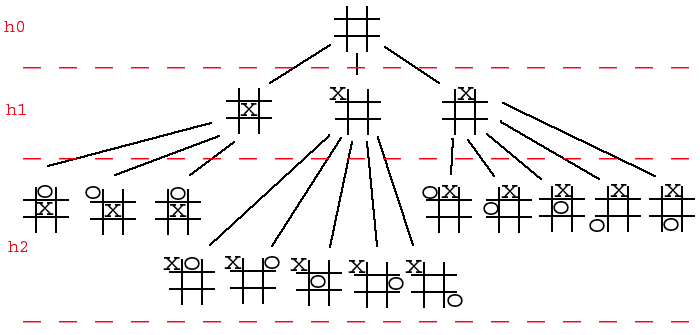
\includegraphics[width=5in]{obrazki/chess_tree.png}
	\caption{Schemat drzewa gry K�ko i Krzy�yk.}
	\label{fig:xo_tree}
\end{figure}

\begin{figure}[!h]
	\centering
	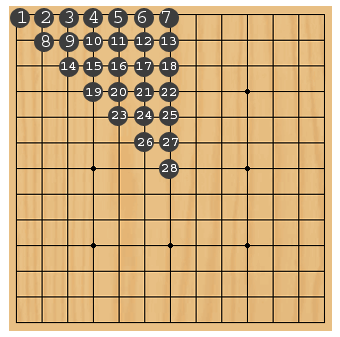
\includegraphics[width=5in]{obrazki/go_tree.png}
	\caption{Przyk�ad pierwszych mo�liwych unikalnych ruch�w w grze GO.}
	\label{fig:go_tree}
\end{figure}

\end{par}
\begin{par}
Je�li chcemy wprowadzi� podzia� gier przydatny przy projektowaniu systemu pierwszym czynnikiem b�dzie typ rozgrywki ze wzgl�du na czas.
Wi�kszo�� gier mo�na podzieli� w�wczas w nast�puj�cy spos�b:
\begin{itemize}
	\item Gry turowe - Gracze naprzemiennie wykonuj� ruchy, przy czym czas na podj�cie decyzji jest relatywnie du�y - od kilku sekund nawet do 1-2 minut.
Wiele nieskomplikowanych gier turowych zosta�o ju� dawno rozwi�zanych przez algorytmy typu minmax, do tego stopnia, �e systemy graj� w nie ju� niemal bezb��dnie. 
W wielu przypadkach przestrze� rozwi�za� jest jednak wci�� zbyt du�a aby zrealizowa� to algorytmem dok�adnym - przyk�adem mo�e by� wy�ej wspomniana gra GO.
	\item Gry czasu rzeczywistego - Gra toczy si� w dynamicznym �rodowisku gry, cz�sto z wieloma obiektami i graczami na raz. Cz�sto czas na podj�cie optymalnej decyzji przez algorytm jest mocno ograniczony - program musi podejmowa� decyzje nawet do 30 razy w ci�gu sekundy. Opr�cz tego pr�ba dyskretyzacji �rodowiska i znalezienia dok�adnego rozwi�zania z przestrzeni stan�w gry jest w praktyce niewykonalna. Przyk�adem mog� by� tutaj r�nego rodzaju dwuwymiarowe lub tr�jwymiarowe gry akcji, kt�re cz�sto posiadaj� z�o�one �rodowiska gry, wiele dynamicznych obiekt�w oraz graczy uczestnicz�cych w rozgrywce poprzez przez sie� komputerow�. Przy projektowaniu sztucznej inteligencji w takim �rodowisku w tej chwili mo�emy liczy� jedynie na wyniki przybli�one.
\end{itemize}
\end{par}
\begin{par}
Sztuczna inteligencja w grach mo�e dotyczy� r�nych aspekt�w gry. 
W grach logicznych (turowych) g��wnym, i jedynym problemem jest podj�cie najlepszej decyzji dla aktualnego stanu gry daj�cej zwyci�stwo. 
W wi�kszo�ci gier logicznych sztuczna inteligencja ma za zadanie symulacj� godnego przeciwnika dla cz�owieka.
Cz�sto jednak te same algorytmy mog� s�u�y� do cel�w edukacyjnych b�d� do podpowiedzi - ten sam system graj�cy w szachy mo�e gra� przeciwko nam, jak i podpowiada� nam ruchy na podstawie naszej pozycji na planszy.
Podobnie wygl�da sytuacja w grach czasu rzeczywistego, jednak problem znacznie si� komplikuje.
Poniewa� przestrze� rozwi�za� jest bardzo du�a, cz�sto podj�cie decyzji mo�e by� wspomagane przez algorytm przybli�ony, b�d� oparty na algorytmach genetycznych.
Algorytm minmax w wi�kszo�ci przypadk�w zawodzi, b�d� jego czas dzia�ania jest zbyt wolny do zastosowania w dynamicznie dzia�aj�cym �rodowisku.
Korzystaj�c z algorytm�w ``jedynie'' optymalizuj�cych rozgrywk� tracimy mo�liwo�� rozegrania idealnej partii gry, jednak cz�sto wystarcza to dla stworzenia godnego przeciwnika dla ludzkich graczy.
\end{par}

\section{Podstawy algorytm�w genetycznych.}
\begin{par}
Cz�sto wykorzystywanym sposobem rozwi�zania z�o�onego problemu algorytmicznego s� algorytmy genetyczne.
Opieraj� si� one na zasadach ewolucji odkrytych przez Charlesa Darwina, i wzoruj� si� na faktycznych rozwi�zaniach doboru naturalnego wyst�puj�cych w przyrodzie.
Algorytm ewolucyjny opiera si� na wprowadzeniu losowego czynnika do ca�ej procedury, i tym te� r�ni si� od klasycznego algorytmu, i� jest niedeterministyczny. 
Og�lny przebieg algorytmu genetycznego mo�e wygl�da� nast�puj�co:
\begin{enumerate}
\item Wygenerowanie pocz�tkowej populacji osobnik�w (propozycji rozwi�za�) w spos�b losowy.
\item Przeliczenie funkcji przystosowania dla ka�dego z osobnik�w.
\item Uporz�dkowanie populacji malej�co wzgl�dem wyniku funkcji przystosowania.
\item Wybranie populacji rodzicielskiej zgodnie z przyj�t� metod� selekcji.
\item Krzy�owanie osobnik�w z populacji rodzicielskiej i otrzymanie nowej populacji - nowe potomstwo posiada cechy rodzic�w kt�rzy w poprzedniej populacji byli najlepiej przystosowani do rozwi�zania danego problemu.
\item Mutacja cz�ci potomstwa - wprowadzenie czynnika losowego poprzez zmian� niekt�rych fragment�w chromosomu w spos�b losowy.
\item Je�li warunek ko�cowy nie zosta� osi�gni�ty powr�t do kroku 2, w przeciwnym wypadku koniec algorytmu.
\end{enumerate}
Wynikiem takiego algorytmu jest nie jedno rozwi�zanie problemu, a ca�a ich populacja.
W wi�kszo�ci algorytm�w genetycznych mo�na wydzieli� kilka koniecznych do zaprojektowania klas b�d� procedur.
\begin{enumerate}
\item Chromosom oraz Populacja
	\begin{par}
		Pierwszym krokiem jest zdefiniowanie typu danych odpowiednich do przetrzymywania informacji o danym osobniku.
		Odpowiednio zaprojektowany format danych (zwany Chromosomem) pozwoli na �atw� implementacj� pozosta�ych element�w oraz zapewni generowanie optymalnych wynik�w.
		Informacja ta cz�sto jest reprezentowana przez tablic� warto�ci, b�d� list� cech przypisanych do danej klasy. 
		Chromosom odpowiada za informacj� o pojedynczym osobniku, natomiast Populacja traktowana jest jako wszystkie osobniki nale��ce do danego zbioru w danej iteracji algorytmu. 
		O ile w podstawowych algorytmach genetycznych Populacja jest jedynie kontenerem, dobrze jest pami�ta� o ewentualnym rozbudowaniu Populacji do bardziej z�o�onej klasy, dzi�ki czemu b�dziemy mieli mo�liwo�� prostego por�wnywania, b�d� zapami�tywania ca�ych populacji.
	\end{par}
\item Funkcja Przystosowania
	\begin{par}
		Kolejnym istotnym krokiem jest zdefiniowanie funkcji przystosowania.
		W doborze naturalnym wyst�puj�cym w przyrodzie, osobniki danego gatunku ro�liny b�d� zwierz�cia r�ni� si� pod wzgl�dem genetycznym. 
		Mo�na w�wczas wywnioskowa� i� cz�� z nich jest lepiej przystosowana do danego �rodowiska, co z kolei wp�ywa na ich szanse prze�ycia w trudnych sytuacjach, liczno�� potomstwa, d�ugo�� �ycia.
		Poniewa� potomstwo dziedziczy geny po swoich rodzicach, ``zwyci�skie'' cechy w kolejnym pokoleniu s� bardziej powszechne.
		Odpowiednikiem funkcji przystosowania jest w�a�nie wynikowa cech danego osobnika kt�ra okre�la prawdopodobie�stwo przekazania jego gen�w w kolejnym pokoleniu.
		Funkcja przystosowania jest do�� prosta w realizacji, o ile dane dotycz�ce osobnika s� �atwe do zmierzenia -- w�wczas mo�e by� to jedynie kwestia policzenia warto�ci funkcji liniowej z odpowiednimi wagami, gdzie argumentami s� wyniki osobnika podczas symulacji w �rodowisku.
		Mimo to w wi�kszo�ci algorytm�w genetycznych dobranie odpowiednich wag w funkcji przystosowania jest kluczowym czynnikiem nad kt�rym p�niej mo�na d�ugo pracowa� przy optymalizacji algorytmu.
	\end{par}
\item Krzy�owanie
	\begin{par}
		Po ka�dym kroku algorytmu zazwyczaj mo�emy uporz�dkowa� osobniki nale��ce do bie��cej populacji i wylosowa� z niej pewien zbi�r osobnik�w najlepiej przystosowanych (wp�yw na to wynik funkcji przystosowania). 
		W�wczas dokonujemy krzy�owania pomi�dzy nimi, dzi�ki czemu otrzymujemy osobniki nowe, jednak posiadaj�ce pewne cechy swoich ``rodzic�w''.
		Krok ten jest kluczowy je�li chcemy osi�ga� coraz lepsze wyniki w kolejnych populacjach, poniewa� od dobrej metody krzy�owania zale�y czy kolejne populacje b�d� lepiej przystosowane do rozwi�zania problemu.
		Z�e zaprojektowanie krzy�owania jest jednym z cz�stszych powod�w osi�gania przez populacj� z�ych wynik�w, zw�aszcza gdy Chromosom ma z�o�on� struktur�.
		Samo krzy�owanie cz�sto r�wnie� posiada czynnik losowy (w klasycznych przyk�adach dotycz�cych krzy�owania si� dw�ch ci�g�w bitowych, losowany jest punkt ��czenia si� dw�ch ci�g�w).
	\end{par}
\item Mutacja
	\begin{par}
		O ile pocz�tkowa losowo�� algorytmu polegaj�ca na wylosowaniu pierwszej populacji jest szybko zast�powana przez populacj� osi�gaj�c� lepsze wyniki, 
		warto w trakcie ca�ego procesu pr�bowa� modyfikowa� kilka osobnik�w, nawet je�li mog�oby to spowodowa� chwilowe pogorszenie populacji. 
		W innym przypadku zbyt uporz�dkowana procedura selekcji i krzy�owania osobnik�w spowoduje stagnacj� populacji.
		Cz�sto mo�na to zauwa�y� gdy po kilku iteracjach wi�kszo��, b�d� ca�a populacja jest identyczna.
		Najcz�stsz� realizacj� mutacji jest zmiana jakiego� parametru (b�d� grupy parametr�w) danego osobnika na warto�� zupe�nie losow�.
		Poniewa� w du�ej mierze zale�y to od budowy Chromosomu, nie ma uniwersalnej metody na zaimplementowanie mutacji.
		Najcz�ciej mutacja wyst�puje z niskim prawdopodobie�stwem,
		\begin{center}
			$p_m < 0.1$
		\end{center}
		tak aby nie ingerowa� zbyt mocno w algorytm. Ostatecznie nale�y d��y� do pewnej systematycznej optymalizacji, a nie tylko polega� na czynniku losowym.
	\end{par}
\item Metoda Selekcji
	\begin{par}
		Sama metoda wyboru populacji rodzicielskiej r�wnie� ma znaczenie, poniewa� jednak jest ona oparta na warto�ci funkcji przystosowania, to ju� sama metoda wyboru ma mniej krytyczne znaczenie.
		Najbardziej popularne metody selekcji to:
		\begin{enumerate}
			\item Metoda ko�a ruletki.
				\begin{par}
					Sama nazwa bierze si� od popularnej gry w ruletk�, w kt�rej pole powierzchni ka�dego wycinka ko�a jest proporcjonalne do prawdopodobie�stwa wylosowania danej liczby. 
					Oczywi�cie w klasycznej ruletce pola wycink�w ko�a s� r�wne, zatem szansa wylosowania ka�dej liczby jest taka sama.
					W samym algorytmie wirtualne ``wycinki ko�a'' nie musz� oczywi�cie by� r�wne. 
					Osobnik kt�ry osi�ga lepsze wyniki w funkcji przystosowania otrzymuje wi�ksze prawdopodobie�stwo w��czenia do populacji rodzicielskiej ni� osobniki s�absze. 
					Aby to zrealizowa� losowana jest pewna warto�� (najcz�ciej z przedzia�u [0,1], liczb wymiernych) kt�ra potem jednoznacznie okre�la kt�ry osobnik zosta� wylosowany.
					Praktycznie realizowane jest to w nast�puj�cy spos�b:
					\begin{center}
						$p(k)=\frac{f(k)}{\displaystyle\sum\limits_{i=0}^n f(i)}$
					\end{center}
					gdzie $p(k)$ oznacza prawdopodobie�stwo wylosowana k-tego osobnika z populacji, a $f(i)$ warto�� funkcji przystosowania i-tego osobnika. Poniewa� warto�ci s� znormalizowane, suma prawdopodobie�stw wylosowania ka�dego z osobnik�w jest r�wna 1.
					Po uporz�dkowaniu osobnik�w, potrzebna jest jedynie losowa warto�� ktora jednoznacznie okre�li wyb�r osobnika.
					
				\end{par}
			\item Metoda rankingowa.
				\begin{par}
					W tej metodzie sortujemy osobniki malej�co wzgl�dem funkcji przystosowania i wybieramy populacj� rodzic�w jako $m$ pierwszych osobnik�w (zwan� cz�sto elit� populacji). 
					Ma to pewn� wad�, gdy� powoduje po pewnym czasie stagnacj� (brak czynnika losowego). 
					Innym wariantem jest selekcja turniejowa w kt�rej najpierw dzielimy grup� na $G$ podgrup spo�r�d kt�rych wybieramy najlepsze osobniki do populacji rodzicielskiej. 
					Otrzymujemy w ten spos�b G rodzic�w, w�r�d kt�rych niekoniecznie s� najlepsze osobniki globalnie (nawet z bardzo silnej grupy przechodzi tylko jeden osobnik). 
					Daje nam to ju� pewn� losowo�� w wyborze populacji rodzicielskiej.
				\end{par}
			\item Po��czenie kilku metod.
				\begin{par}
					Dodatkowym elementem mo�e by� po��czenie kilku metod selekcji celem otrzymania najbardziej optymalnej selekcji dla danego problemu genetycznego. 
					W zasadzie bardziej z�o�one problemy ewolucyjne wr�cz wymagaj� w�asnej inwencji do zaprojektowania dobrego systemu.
				\end{par}
		\end{enumerate}
	\end{par}
\end{enumerate}
	Du�� cz�ci� dobrego systemu genetycznego jest odpowiednia mo�liwo�� konfiguracji danych odpowiadaj�cych za ka�dy z krok�w.
	Mamy dzi�ki temu mo�liwo�� przetestowania r�nych podej�� do danego problemu bez bezpo�rednich i cz�sto uci��liwych zmian w kodzie programu.
	Opr�cz tego ca�y proces mo�na zautomatyzowa�, dzi�ki czemu mo�emy w prosty spos�b przetestowa� algorytm dla r�nych danych konfiguracyjnych.
\end{par}

\chapter{Analiza wymaga�}
Przed implementacj� systemu nale�y przeprowadzi� analiz� problemu, okre�li� wymagania systemu, zadecydowa� o narz�dziach i technologiach niezb�dnych w implementacji systemu.
W tym rozdziale zostan� opisane koniecznie do zaimplementowania modu�y oraz postawione zostan� wymagania jakie system musi spe�nia�. Pierwszym krokiem b�dzie om�wienie narz�dzi i technologii koniecznych do implementacji systemu.


\section{Wykorzystane narz�dzia i j�zyki programowania}
\begin{par}
	\subsection{J�zyk Java}
	G��wnym celem do zrealizowania w pracy jest problem algorytmiczny i teoretyczny.
	Praca w mniejszym stopniu opiera si� na wykorzystaniu konkretnej technologii, czy j�zyka programowania, wobec czego zosta�y wykorzystane popularne narz�dzia i j�zyki programowania.
	System zosta� napisany w j�zyku Java oraz testowany na wirtualnej maszynie javy w wersji Java SE 7u2. 
	Java jest j�zykiem programowania wysokiego poziomu zaprojektowanym i stworzonym przez Jamesa Groslinga podczas gry pracowa� w firmie Sun Microsystems. Pierwsza propozycja stworzenia Javy pojawi�a si� w roku 1991, do g��wnych tw�rc�w opr�cz Jamesa Groslinga zalicza si� r�wnie� Mike'a Sheridana oraz Patrick'a Naughtona.
	Pocz�tkowo j�zyk Java by� bezpo�rednio zwi�zany z firm� Sun Microsystems, kt�ra kontrolowa�a jego rozw�j do roku 2010.
	Od tego czasu firma Sun sta�a si� cz�ci� korporacji Oracle, wobec czego wszelkie prawa zwi�zane z j�zykiem Java posiada Oracle.
	Java swoj� sk�adni� przypomina j�zyk C, aczkolwiek w�r�d pierwowzor�w wymienia si� r�wnie� j�zyk Smalltalk.
	Aplikacje napisane w j�zyku Java s� kompilowane do kodu bajtowego Javy (ang. java bytecode), i uruchamiane na maszynie wirtualnej, co zapewnia pewnego rodzaju bezpiecze�stwo w stosunku do j�zyka C lub C++.
	Inn� du�� zalet� j�zyka Java jest jego przeno�no��.
	Jedynym wymogiem uruchomienia aplikacji javowej na dowolnym systemie jest obecno�� wirtualnej maszyny javy (ang. JVM - Java Virtual Machine).
	Dzi� wi�kszo�� urz�dze� mobilnych posiada wirtualn� maszyn� javy pozwalaj�c� na uruchamianie aplikacji napisanych w tym j�zyku.
	Jak pisze Bruce Eckel w swojej ksi��ce po�wi�conej j�zykowi Java: ``To, co wywar�o na mnie najwi�ksze wra�enie, kiedy poznawa�em jav�, to fakt, �e w�r�d innych cel�w projektant�w z firmy Sun znalaz�a si� tak�e redukcja z�o�ono�ci dla programisty. 
	To tak, jakby powiedzie�: ``Nie dbamy o nic poza zmniejszeniem czasu i trudno�ci tworzenia porz�dnego kodu.''(...)''.\cite[str. 19-20]{ThinkingJava}
	Poniewa� cz�� algorytmiczna aplikacji wymaga przeprowadzania cz�stych symulacji zachowania �rodowiska oraz przeprowadzania ca�ego przebiegu gry, istotnym czynnikiem by� czas dzia�ania krytycznych miejsc w aplikacji - g��wnie p�tli gry, wy�wietlania oraz generowania nowej populacji na podstawie poprzedniej.
	Java jako j�zyk polegaj�cy na maszynie wirtualnej posiada warstw� po�redni� kt�ra spowalnia ca�y proces i jest wolniejsza od j�zyka C lub C++, jednak prostota realizacji cz�ci wizualnej aplikacji oraz bardzo dobra przeno�no�� przewa�y�y w wyborze j�zyka.
	Kolejnym trafnym wyborem je�li chodzi o j�zyk i narz�dzia by�by prawdopodobnie C++ wraz z bibliotek� Qt do generowania grafiki, tworzenia okien oraz kontrolek.
	T� sam� aplikacj� mo�na by zrealizowa� za pomoc� j�zyka Python i biblioteki PyGame/Qt do warstwy wizualizacyjnej, jednak w�wczas koszt czasowy realizacji algorytmu genetycznego oraz logiki gry m�g�by okaza� si� znacz�co du�y. Wynika to z faktu i� Python jest j�zykiem interpretowanym, i generalnie nie jest przeznaczony do du�ych oblicze�. Mimo to, przy konieczno�ci realizacji prostej wersji demonstracyjnej programu opisywanego w pracy, j�zyk Python wraz z bibliotek� PyGame mo�e okaza� si� najszybszym do implementacji ze wzgl�du na kr�tki kod, dynamiczne typy zmiennych oraz bogat� kolekcj� struktur takich jak listy czy mapy incydencji konieczne do realizacji algorytmu.
	Sama aplikacja korzysta z kolekcji i podstawowych struktur danych wyst�puj�cych w j�zyku Java.
	\subsection{Biblioteka Swing}
	Biblioteka Swing zosta�a u�yta do stworzenia warstwy wizualnej programu.
	Pierwsz� pr�b� stworzenia biblioteki graficznej javy pozwalaj�cej na tworzenie graficznego interfejsu u�ytkownika by�a biblioteka AWT (ang. Abstract Window Toolkit).
	Fala niezadowolenia w�r�d programist�w sprawi�a i� ograniczone i ma�o efektowne elementy graficzne biblioteki AWT zosta�y zast�pione przez zbi�r komponent�w dzi� znanych jako Swing.
	W bibliotece Swing znajdziemy wi�kszo�� podstawowych komponent�w wyst�puj�cych we wsp�czesnych systemach operacyjnych w��cznie z obs�ug� okien, natomiast w bibliotece AWT znajdziemy obs�ug� zdarze�, co w po��czeniu daje nam wystarczaj�ce narz�dzia do stworzenia graficznego interfejsu.
	Warto zauwa�y� i� Swing nie korzysta z domy�lnych ustawie� systemu je�li chodzi o wygl�d komponent�w, dzi�ki czemu ten sam program wygl�da identycznie na ka�dym systemie operacyjnym.
	Wi�cej informacji o bibliotece Swing jak i j�zyku Java mo�na znale�� w ksi��ce Thinking in Java \cite[rozdz. 22. Graficzne interfejsy u�ytkownika]{ThinkingJava}.
	Alternatyw� dla biblioteki Swing mo�e by� biblioteka SWT zwi�zana z projektem Eclipse.
	W odr�nieniu do Swing, komponenty korzystaj� z wygl�du komponent�w systemu operacyjnego, dzi�ki czemu mo�liwe jest uzyskanie wygl�du pasuj�cego do danego systemu operacyjnego. Biblioteka SWT jest darmowa i dost�pna na stronie domowej projektu Eclipse \cite{swt}.
	\subsection{Narz�dzia}
	Aplikacja w ca�o�ci zosta�a zrealizowana w programie Netbeans 6.9.1 wspieraj�cym testowanie, kompilacj� i budowanie aplikacji napisanych w j�zyku Java.
	Projekt NetBeans jako narz�dzie by� pocz�tkowo rozwijany przez Romana Staneka od roku 1996 a� do roku 1999 kiedy to NetBeans zosta� on zakupiony przez firm� Sun Microsystems. Rok p�niej udost�pniony zosta� kod �r�d�owy programu. Do dzisiaj jest on rozwijany przez wielu programist�w z ca�ego �wiata. Aktualna wersja to NetBeans 7.0.1, dost�pna od 1 Sierpnia 2011 roku. Aplikacja NetBeans wraz z dokumentacj� jest darmowa i dost�pna na stronie domowej projektu \cite{netbeans}
	Innym popularnym narz�dziem jest program Eclipse. Z punktu widzenia programisty r�nica pomi�dzy narz�dziami jest nieznaczna i w g��wnej mierze zale�y od preferencji.
\end{par}
\section{Wst�pna analiza problemu}
\begin{par}
	\subsection{Sterowanie}
	\begin{par}
	Aby zrealizowa� cz�� odpowiedzialn� za sterowanie postaci�, nale�y u�y� klasy po�redniej pomi�dzy warstw� logiki silnika gry, a warstw� komunikacji z graczem.
	Przy takim rozwi�zaniu sygna�y z klawiatury b�d� innych urz�dze� peryferyjnych s� przekazywane do warstwy po�rednicz�cej.
	Dzi�ki takiemu wyj�ciu mo�emy �atwo zmieni� �r�d�o sygna��w trafiaj�cych do postaci z bezpo�rednich wci�ni�� klawiszy na akcje przechowywane w chromosomie.
	Warstwa po�rednia odpowiada w�wczas za sterowanie postaci� gracza w taki sam usystematyzowany spos�b, niezale�nie od �r�d�a sygna��w. 
	Z punktu widzenia logiki gry nie ma r�nicy pomi�dzy sygna�ami z klawiatury, a wygenerowanymi akcjami.
	\end{par}
	
	\subsection{Projekt chromosomu}
	Kolejnym wa�nym elementem jest odpowiednie zaprojektowanie struktury chromosomu. 
	Dwa najbardziej trafne rozwi�zania opieraj� si� na dw�ch zmiennych wyst�puj�cych w �rodowisku gry: czasie oraz pozycji gracza.
	\begin{enumerate}
	\item
	{\bf Czas kt�ry up�yn�� od rozpocz�cia danej instancji przej�cia. }
	\begin{par}

		To rozwi�zanie zak�ada podejmowanie akcji w grze w zale�no�ci od czasu kt�ry up�yn�� od jej rozpocz�cia.
		Warto zauwa�y� i� nie jeste�my ograniczeni po�o�eniem postaci na planszy, dzi�ki czemu mo�liwe s� takie operacje jak brak akcji, czy powr�t do pocz�tku planszy je�li to korzystne.
		Istotn� wad� tego rozwi�zania by�aby du�a podatno�� algorytmu na zap�tlanie si�, lub wykonywanie du�ej ilo�ci ma�o przydatnych ruch�w. 
		Mo�na �atwo zauwa�y� �e przy r�wnym prawdopodobie�stwie ruchu w lewo i prawo, posta� tylko nieznacznie b�dzie oddala� si� punktu startowego. 
		Prostym rozwi�zaniem tego problemu jest przyporz�dkowanie pewnego prawdopodobie�stwa ka�dej akcji, dzi�ki czemu mo�emy za�o�y� �e preferowanym kierunkiem jest np. ruch postaci w prawo, nie trac�c mo�liwo�ci minimalnego ruchu w lewo je�li to korzystne.
		Pewnym utrudnieniem mo�e by� krzy�owanie tego typu chromosom�w. Poniewa� akcje postaci w wi�kszo�ci przypadk�w maj� sens w kontek�cie jej aktualnego po�o�enia, o tyle klasyczne krzy�owanie poprzez ''ci�cia'' chromosomu na dwie cz�ci mo�e okaza� si� kosztowne.
		Wybranie losowego punktu przeci�cia i z��czenie ze sob� dw�ch chromosom�w nie jest dobrym rozwi�zaniem.
		Po po��czeniu otrzymamy niesp�jny ci�g ruch�w, kt�re b�d� mia�y niewiele wsp�lnego z aktualn� pozycj� gracza na mapie, wobec czego b�d� nieu�yteczne.
		Mo�na temu zapobiec zapewniaj�c ��czenie si� chromosom�w jedynie w punktach w kt�rych posta� w obu momentach znajduje si� w tym samym lub zbli�onym miejscu. Wyznaczenie takich punkt�w mo�e okaza� si� kosztowne.
		Przeszukiwanie punkt�w wsp�lnych mo�na zrealizowa� w czasie $O(n*log_2n)$ najpierw sortuj�c tablice obu osobnik�w odpowiadaj�ce za ruch w chromosomie. 
		Tablice sortujemy wzgl�dem wsp�rz�dnej X aktualnego po�o�enia gracza dla ka�dej z akcji, a nast�pnie liniowo przechodz�c po obu tablicach osobnik�w, szukaj�c punkt�w wsp�lnych.
		W�wczas wida� i� trzeba przechowywa� dane na temat po�o�enia w chromosomie, co jest nieco niesp�jne z ide� poruszania si� wzgl�dem czasu.
		Wst�pny schemat takiego rozwi�zania m�g�by w�wczas wygl�da� tak jak na rysunku \ref{fig:sterowanie}.
		
		\begin{figure}[!h]
		\centering
		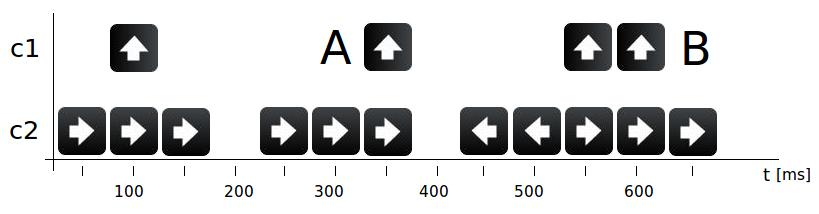
\includegraphics[width=\textwidth]{obrazki/sterowanie.jpg}
		\caption{Sterowanie wzgl�dem czasu.}
		\label{fig:sterowanie}
		\end{figure}
		
		Tablice c1, c2 oznaczaj� odpowiednio tablic� odpowiadaj�c� za akcje specjalne (np. skok), oraz tablic� odpowiadaj�c� jedynie za ruch kierunkowy.

		Lepszym rozwi�zaniem jest realizacja krzy�owania nie poprzez klasyczne podej�cie, lecz modelowane statystycznie: Potomstwo nie otrzymuje bezpo�rednich fragment�w chromosomu, lecz losuje za ka�dym razem nowe ruchy,
		natomiast chromosomy populacji rodzicielskiej zwi�kszaj� prawdopodobie�stwo wylosowania najcz�ciej wyst�puj�cych ruch�w.
		Schemat takiego rozwi�zania zaprezentowany jest na Rys. \ref{fig:krzy�owanie}, gdzie przedstawione zosta�o krzy�owanie populacji sk�adaj�cej si� z 3 osobnik�w (p1,p2,p3) oraz spos�b liczenia nowych prawdopodobie�stw w danym punkcie chromosomu.
		Do tego rozwi�zania w��czamy sta�� decyduj�c� o wadze jakie ma krzy�owanie: Je�li rodzic posiada pewn� akcj� A w pewnym miejscu swojego chromosomu,
		w�wczas potomkowi losowana jest nowa akcja, z t� r�nic� i� akcja A ma teraz prawdopodobie�stwo wylosowania $p_A = p_A + p_A*k$. Je�li populacja rodzicielska sk�ada si� z $n$ rodzic�w,
		oraz $m$ z nich posiada w danym momencie tak� sam� akcj� w�wczas nowe prawdopodobie�stwo wylosowania akcji (tylko dla tego rozpatrywanego miejsca) wynosi 
		\begin{center}
		$p_A =  p_A + {\displaystyle\sum\limits_{i=1}^m (p_A*k)} = p_A + (p_A*k)*m$.
		\end{center}
		Dzi�ki takiemu podej�ciu zachowujemy ide� krzy�owania oraz znacznie upraszczamy ca�y proces. Warto�ci prawdopodobie�stw na koniec s� normalizowane aby dawa� w sumie warto�� 1.
		
		\begin{figure}[!h]
		\centering
		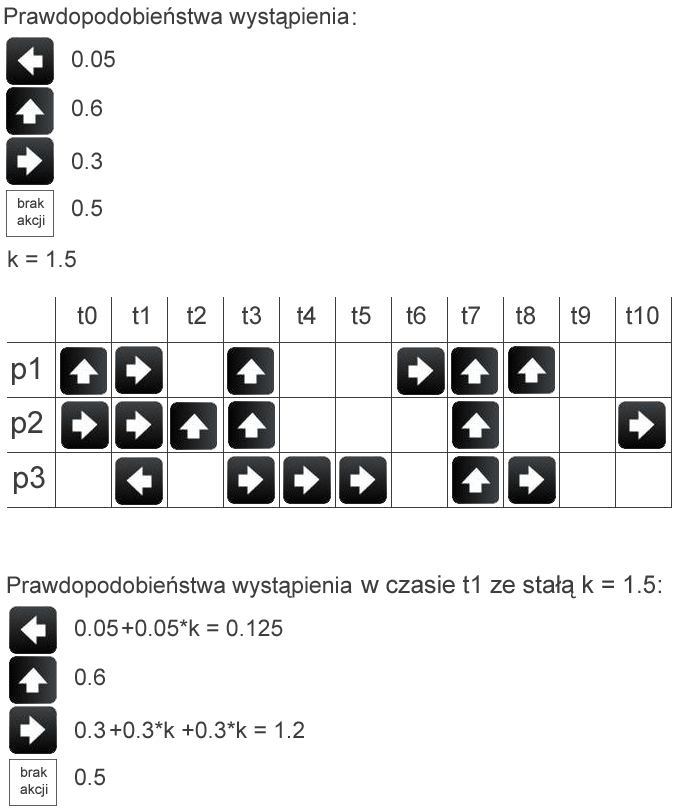
\includegraphics[width=5in]{obrazki/stat_cross.png}
		\caption{Krzy�owanie modelowane statystyczne.}
		\label{fig:krzy�owanie}
		\end{figure}

	\end{par}
	\item
	{\bf Aktualna pozycja gracza.}
	\begin{par}
		O ile poprzednie rozwi�zanie dawa�o wi�ksz� swobod� ruchu po mapie, to by�o jednak ma�o optymalne pod wzgl�dem osi�gania szybko dobrych wynik�w.
		Je�li za�o�ymy i� akcje przechowywane w chromosomie maj� by� aktywowane w momencie osi�gni�cia przez gracza danej pozycji na osi X mapy, w�wczas upro�cimy ca�y mechanizm krzy�owania (ju� nie musimy szuka� punkt�w wsp�lnych, gdy� dwa dowolne indeksy w obu tablicach $i,j$ gwarantuj� nam takie samo po�o�enie gracza na mapie gdy $i=j$.
		Opr�cz tego przy za�o�eniu �e plansz� da si� rozwi�za� poruszaj�c si� tylko w prawo upraszcza to wi�kszo�� operacji w algorytmie.
		Innym udogodnieniem b�dzie uproszczenie samego typu przechowywanych danych. Poniewa� rezygnujemy z postoj�w i ruchu w lewo, r�wnie dobrze mo�emy zrezygnowa� z tablicy przechowuj�cej te informacje.

		\begin{par}
		\begin{figure}[!h]
		\centering
		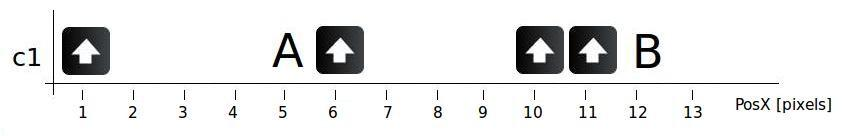
\includegraphics[width=\textwidth]{obrazki/sterowanie2.jpg}
		\caption{Sterowanie wzgl�dem pozycji gracza.}
		\label{fig:sterowanie2}
		\end{figure}
		\end{par}

		To podej�cie posiada jednak kilka powa�nych wad i wymaga pewnych ograniczaj�cych za�o�e�.
		Plansza musi by� ukierunkowana, i by� rozwi�zywalna przy ci�g�ym ruchu w okre�lonym kierunku.
		Jest to rozwi�zanie dzia�aj�ce jedynie dla bardzo w�skiej grupy gier platformowych (np. wspomniane wcze�niej Super Mario Brothers).
		Przeniesienie systemu do zastosowania w grze platformowej o nieco innym schemacie ruchu (np. rozwi�zywania labiryntu) mo�e okaza� si� trudne i wymagaj�ce du�ych zmian w samym algorytmie.
		Jednym z za�o�e� pracy jest unikni�cie takiego podej�cia i traktowanie system bardziej og�lnie, wobec czego obowi�zuj�c� struktur� chromosomu b�dzie ta opisana w pierwszym punkcie.
		
	\end{par}
	\end{enumerate}
	\FloatBarrier
\end{par}
\section{Modu� silnika i symulatora gry}
Poniewa� system mo�na podzieli� na dwa g��wne modu�y (symulacji oraz edytora map) zostan� one rozpatrzone oddzielnie.
W tym rozdziale zostanie przeprowadzona analiza wymaga� modu�u odpowiadaj�cego za symulacj� �rodowiska gry oraz przeprowadzanie treningu populacji algorytmem genetycznym.

\subsection{Wymagania funkcjonalne}
	System nie wymaga r�nicowania u�ytkownik�w ze wzgl�du na role. Wymagania funkcjonalne wygl�daj� nast�puj�co:
	\begin{itemize}
		\item {\bf Poruszanie si� w �rodowisku gry za pomoc� klawiatury.}
		\newline
		Podstawowym wymogiem systemu jest implementacja silnika prostej gry platformowej pozwalaj�cego na poruszanie si� postaci� po mapie.
		Sterowanie zrealizowane powinno by� intuicyjne i analogiczne do przyj�tych rozwi�za� w grach platformowych.
		Poniewa� oprawa graficzna nie jest priorytetem w projekcie, wystarczy prosta reprezentacja obiekt�w za pomoc� prostok�t�w.
		\item {\bf Wczytanie mapy do �rodowiska gry.}
		\newline
		System powinien pozwala� na wczytywanie map z plik�w tekstowych do bie��cego �rodowiska symuluj�cego przebieg gry.
		W�wczas bie��ca gra zostaje przerwana i inicjowany jest nowy przebieg gry na nowo wczytanej mapie.
		\item {\bf Wczytanie nowej logiki do �rodowiska gry.}
		\newline
		Poniewa� system powinien by� og�lnym systemem rozwi�zuj�cym gry platformowe, dost�pnych powinno by� kilka przyk�adowych gier,
		r�ni�cych si� mi�dzy sob� pod wzgl�dem logiki. Podobnie jak w powy�szym przypadku bie��ca gra powinna zosta� przerwana i
		powinien zosta� zainicjowany nowy przebieg gry z now� logik�.
		\item {\bf Przej�cie w tryb treningu populacji.}
		\newline
		Po przej�ciu w tryb treningu populacji u�ytkownikowi odbierana jest mo�liwo�� poruszania si� postaci� po ekranie.
		Je�li nie istnieje jeszcze zainicjowana �adna populacja pocz�tkowa, nast�puje wylosowanie pierwszej populacji, po czym system rozpoczyna trening populacji w danym �rodowisku gry, zgodnie z danymi ustawieniami w systemie. Przechodzenie pomi�dzy treningiem populacji a gr� u�ytkownika powinno by� mo�liwe w obie strony. 
		W�wczas je�li u�ytkownik zainicjuje trening populacji, nast�pnie przejdzie w tryb swobodnej gry, a ostatecznie znowu rozpocznie trening populacji, domy�ln� populacj� jest ta kt�ra zosta�a zapisana podczas ostatniego treningu.
		\item {\bf Zainicjowane nowej populacji. }
		\newline
		Mo�e okaza� si� koniecznie zainicjowanie nowej populacji podczas dzia�ania systemu, np. gdy populacja wpad�a w stagnacj�.
		Inicjowanie nowej populacji podczas zmiany logiki, ustawie� b�d� wczytywania mapy jest realizowane automatycznie.
		\item {\bf Otworzenie okna ustawie�.}
		\newline
		System ze wzgl�du na warstw� genetyczn� powinien by� w �atwo konfigurowalny. Po wy�wietleniu okna ustawie� u�ytkownik ma mo�liwo�� zmiany
		poszczeg�lnych parametr�w algorytmu b�d� symulacji gry.
		\item {\bf Zastosowanie nowych ustawie�. }
		\newline
		Poniewa� niekt�re ustawienia wymagaj� porzucenia aktualnego wyniku populacji i rozpocz�cia symulacji od pocz�tku (np. rozmiar chromosomu).
		U�ytkownik jest o tym fakcie informowany i pytany o ponownie uruchomienie algorytmu. 
		W przypadku gdy nie jest to koniecznie, algorytm nie zostaje przerwany, a u�ytkownik wedle woli mo�e to uczyni� w�asnor�cznie.
		\item {\bf Otworzenie okna populacji. }
		\newline
		Podczas dzia�ania algorytmu powinien by� mo�liwy podgl�d aktualnej populacji. U�ytkownikowi widoczna jest w�wczas lista osobnik�w, oraz kr�tki opis ka�dego z nich:
		Wynik ko�cowy, ilo�� zebranych punkt�w, czas dzia�ania, warto�� funkcji przystosowania. Dodatkowym elementem jest mo�liwo�� przerwania aktualnego przebiegu gry i uruchomienie tymczasowo nowego przebiegu dla dowolnego osobnika z listy wybranego przez u�ytkownika. Po zako�czeniu przebiegu algorytm powraca do treningu populacji.
		\item {\bf Otworzenie okna osobnika. }
		\newline
		Bezpo�rednio z okna populacji u�ytkownik ma mo�liwo�� podejrzenia szczeg��w dotycz�cych osobnik�w. W�wczas otwierane jest nowe okno zawieraj�ce wszystkie informacje na temat danego osobnika takie jak d�ugo�� tablicy chromosomu b�d� tekstowa reprezentacja ca�ego chromosomu.		
		\item {\bf Przyspieszenie pracy algorytmu.}
		\newline
		Podczas treningu populacji cz�sto niepotrzebne jest u�ytkownikowi �ledzenie ruch�w algorytmu szczeg�lnie w pocz�tkowym stadium. Aby szybciej osi�gn�� wyniki dzia�ania algorytmu rozgrywka jest przyspieszana przez wstrzymanie wy�wietlania grafiki na mapie. Opr�cz tego op�nienie koniecznie do osi�gni�cia 60 klatek na sekund� podczas wy�wietlania zostaje wy��czone - algorytm w tle przeprowadza symulacje.
	\end{itemize}
\subsection{Wymagania niefunkcjonalne}
	\begin{itemize}
	\item {\bf Pr�dko�� dzia�ania aplikacji. }	
	\newline
	Poniewa� aplikacja wymaga przeprowadzenia wielu symulacji gry do osi�gni�cia wyniku, koniecznie jest optymalne zaprojektowanie funkcji bior�cych udzia� w dzia�aniu algorytmu genetycznego.
	\item {\bf Elastyczno��. }
	\newline
	System powinien by� napisany w taki spos�b aby mo�liwe by�o go p�niejsze rozwijanie, szczeg�lnie je�li chodzi o rozszerzanie systemu o nowe logiki gier.
	System musi zosta� rozpatrzony jako generalny system rozwi�zuj�cy gry czasu rzeczywistego opieraj�ce si� na 4 klawiszach kierunkowych i do 4 klawiszy specjalnych.
	\item {\bf Oprawa Graficzna. }
	\newline
	Oprawa graficzna samej gry nie jest istotna w systemie. Je�li system ma by� elastyczny w kwestii mechaniki gry, wprowadzenie bogatej grafiki niepotrzebne skomplikuje proces dodawania nowego typu gry do systemu. 
	Innym powodem zachowania prostej grafiki jest swoboda rozmiar�w obiekt�w. 
	W wi�kszo�ci gier platformowych stosowana jest grafika rastrowa kt�ra przy skalowaniu obiekt�w bez zachowania proporcji wygl�da �le.
	Rozwi�zanie tego problemu wi�za�oby si� z generowaniem grafiki proceduralnie b�d� u�ywaniem grafiki wektorowej, co jednak odbiega od istoty pracy.
	\end{itemize}


\subsection{Diagram przypadk�w u�ycia}
\begin{par}
	Diagram przypadk�w u�ycia zosta� przedstawiony na Rys. \ref{fig:diagram_przypadkow}.
		\begin{figure}[!h]
		\centering
		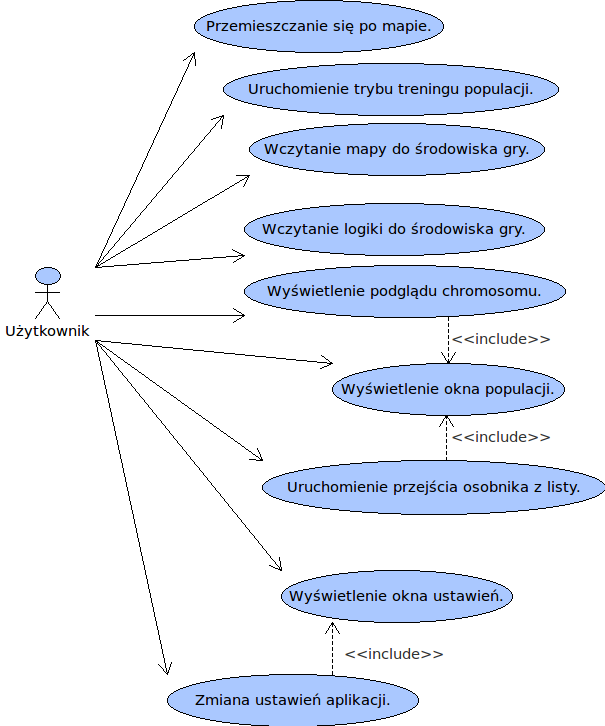
\includegraphics[width=\textwidth]{obrazki/diagram_przypadkow.png}
		\caption{Diagram przypadk�w u�ycia.}
		\label{fig:diagram_przypadkow}
		\end{figure}
		\FloatBarrier
\end{par}
\subsection{Opis tekstowy przypadk�w u�ycia}
\begin{par}
	We wszystkich przypadkach u�ycia aktorem jest u�ytkownik aplikacji.
	\begin{itemize}

	\item
	Opis przypadku u�ycia {\bf Przemieszczanie si� po mapie }.
	\begin{enumerate}
	\item Podstawowy ci�g zdarze�:
		\begin{enumerate}
		\item Po uruchomieniu instancji gry w g��wnym oknie aplikacji wy�wietlona zostaje mapa wraz ze znajduj�cymi si� na niej obiektami.
		\item U�ytkownik za pomoc� klawiszy na klawiaturze przesy�a dane dotycz�ce ruchu i akcji specjalnych do �rodowiska gry.
		\item Posta� gracza znajduj�ca si� w grze reaguje na ��dane akcje, logika gry decyduje o reakcjach obiekt�w w �rodowisku na post�py gracza.
		\item Gracz wchodzi w kolizj� z jednym z obiekt�w ko�cz�cych gr� z danym wynikiem pozytywnym b�d� negatywnym.
		\item Po zako�czeniu gry mapa jest ponownie wczytywana i automatycznie rozpoczynana jest nowa instancja gry.
		\end{enumerate}
	\item Alternatywne ci�g zdarze�:
		\begin{enumerate}
		\item U�ytkownik w trakcie gry uruchamia tryb treningu populacji.
		\item U�ytkownik w trakcie gry wczytuje now� map�, b�d� now� logik� gry, przez co gra jest przerywana i rozpoczynana od nowa.
		\end{enumerate}
	\item Zale�no�ci czasowe:
		\begin{enumerate}
		\item Cz�stotliwo�� wykonania: Samo przemieszczanie si� po mapie jest akcj� o charakterze ci�g�ym. 
		Rozpoczynanie akcji poruszania si� po mapie ze stanu treningu populacji jest bli�ej nieokre�lone, lecz mo�e by� wykonywane �rednio 1-2 razy na minut� dzia�ania aplikacji.
		\item Typowy czas realizacji: 1 minuta.
		\item Maksymalny czas realizacji: nieokre�lony.
		\end{enumerate}
	\item Warto�ci uzyskiwane przez aktor�w po zako�czeniu przypadku u�ycia:
		\begin{enumerate}
		\item Je�li u�ytkownik zako�czy tryb poruszania si� po mapie przez prze��czenie na tryb treningu populacji, w�wczas traci kontrol� nad postaci� i nie ma wp�ywu na akcje rozgrywane w �rodowisku gry.
		\end{enumerate}
	\end{enumerate}
	\item
	Opis przypadku u�ycia {\bf Uruchomienie trybu treningu populacji. }.
	\begin{enumerate}
	\item Podstawowy ci�g zdarze�:
		\begin{enumerate}
		\item Podczas dzia�ania aplikacji gracz uruchamia tryb treningu populacji.
		\item Je�li jest to pierwsze uruchomienie trybu treningu, nie �adna wcze�niej zdefiniowana populacja. W�wczas losowana jest populacja pocz�tkowa w spos�b losowy. W przeciwnym wypadku, symulacja zaczyna si� od ostatniej populacji wygenerowanej przez system. 
		\item System kolejno przeprowadza wszystkie kroki algorytmu genetycznego na bie��cej populacji.
		\item Je�li wy�wietlone jest okno widoku populacji jest ono aktualizowane po ka�dym przebiegu gry.
		\end{enumerate}
	\item Alternatywne ci�g zdarze�:
		\begin{enumerate}
		\item U�ytkownik wybiera w oknie populacji osobnika i przeprowadza jego tymczasow� symulacj� w �rodowisku, przez co trening jest chwilowo wstrzymany. Po symulacji gry danego osobnika trening jest wznawiany od ostatniego osobnika.
		\item U�ytkownik wczytuje now� logik� b�d� map�, przez co aktualny przebieg gry jest przerywany. Zostaje uruchomiona nowa gra i trening populacji jest automatycznie uruchamiany od pocz�tku.
		\item U�ytkownik zmienia ustawienia algorytmu genetycznego. Je�li s� to zmiany wymagaj�ce ponownego uruchomienia gry jest wy�wietlony komunikat potwierdzaj�cy operacj�, w innym wypadku zmiany nast�puj� bez zaburzania aktualnego przebiegu treningu.
		\item U�ytkownik uruchamia tryb przyspieszonego treningu, przez co wy��czona zostaje aktualizacja stanu gry w oknie aplikacji.
		\end{enumerate}
	\item Zale�no�ci czasowe:
		\begin{enumerate}
		\item Cz�stotliwo�� wykonania: Prze��czanie na trening populacji mo�e by� �rednio uruchamiane 1-2 razy w ci�gu minuty dzia�ania aplikacji. 
		\item Typowy czas realizacji: 10 sekund - 5 minut. Samo dzia�anie treningu populacji stanowi� mo�e oko�o 90\% czasu dzia�ania aplikacji.
		\item Maksymalny czas realizacji: nieokre�lony.
		\end{enumerate}
	\item Warto�ci uzyskiwane przez aktor�w po zako�czeniu przypadku u�ycia:
		\begin{enumerate}
		\item Je�li u�ytkownik uruchomi tryb poruszania si� po mapie w�wczas przywr�cone zostaje wy�wietlanie stanu gry (je�li by� w��czony tryb przyspieszonego treningu). U�ytkownik uzyskuje kontrol� nad postaci� gracza.
		\end{enumerate}
	\end{enumerate}
	
	\item
	Opis przypadku u�ycia {\bf Zmiana ustawie� aplikacji. }.
	\begin{enumerate}
	\item Podstawowy ci�g zdarze�:
		\begin{enumerate}
		\item U�ytkownik wy�wietla okno ustawie� aplikacji.
		\item W polach tekstowych u�ytkownik dokonuje zmian na poszczeg�lnych parametrach aplikacji
		\item U�ytkownik zatwierdza zmiany przyciskiem.
		\item System sprawdza czy zmiany nie wymagaj� przerwania bie��cej gry i ponownego uruchomienia algorytmu.
		\begin{enumerate}
			\item Je�li zmiany nie wymagaj� ponownego uruchomienia algorytmu, zmiany zostaj� wprowadzone bez przerywania bie��cej instancji gry.
			\item W wypadku gdy ponowne uruchomienie jest koniecznie wy�wietlone zostaje okno dialogowe.
			U�ytkownik jest pytanie o ponowne uruchomienie algorytmu, ma w�wczas on do dyspozycji zgod� na operacj�, b�d� cofni�cie zmian wymagaj�cych ponownego uruchomienia.
			\item Po podj�ciu decyzji okno dalej pozostaje otwarte, a zgodnie z wyborem zmiany zostaj� dokonane b�d� nie.
		\end{enumerate}
		\item U�ytkownik dalej mo�e dokonywa� zmian ustawieniach aplikacji.
		\end{enumerate}
	\item Alternatywne ci�g zdarze�:
		\begin{enumerate}
		\item U�ytkownik dokonuje zmian, lecz zamiast zatwierdzi� je przyciskiem - zamyka okno ustawie�. W�wczas po ponownym otwarciu �adowane s� aktualne ustawienia a zmiany wprowadzone przez u�ytkownika nie s� zapami�tywane.
		\end{enumerate}
	\item Zale�no�ci czasowe:
		\begin{enumerate}
		\item Cz�stotliwo�� wykonania: 0-5 razy w ci�gu dzia�ania aplikacji.
		\item Typowy czas realizacji: 1 minuta.
		\item Maksymalny czas realizacji: nieokre�lony.
		\end{enumerate}
	\item Warto�ci uzyskiwane przez aktor�w po zako�czeniu przypadku u�ycia:
		\begin{enumerate}
		\item brak
		\end{enumerate}
	\end{enumerate}

	\item
	Opis przypadku u�ycia {\bf Wy�wietlenie podgl�du populacji. }.
	\begin{enumerate}
	\item Podstawowy ci�g zdarze�:
		\begin{enumerate}
		\item Podczas treningu populacji u�ytkownik z menu w oknie g��wnym gry wybiera opcj� ``Population''.
		\item Okno zostaje wy�wietlone, i utworzony zostaje komponent JList wype�niony aktualnymi osobnikami z populacji.
		\item Je�li dany osobnik na li�cie ju� przeprowadzi� symulacj�, widoczne s� warto�ci punktowe zdobyte przez danego osobnika, czas przej�cia oraz wynik ko�cowy.
		\item Podczas dzia�ania algorytmu lista jest automatycznie aktualizowana.
		\item U�ytkownik zamyka okno populacji.
		\end{enumerate}
	\item Alternatywne ci�g zdarze�:
		\begin{enumerate}
		\item U�ytkownik zaznacza osobnika i wy�wietla o nim szczeg�y.
		\begin{enumerate}
			\item Uruchamiany jest przypadek u�ycia ``Wy�wietlenie podgl�du chromosomu''.
		\end{enumerate}
		\item U�ytkownik zaznacza osobnika i uruchamia jego przej�cie gry.
		\begin{enumerate}
			\item Uruchamiany jest przypadek u�ycia ``Uruchomienie przej�cia osobnika z listy.''.
		\end{enumerate}
		\end{enumerate}
	\item Zale�no�ci czasowe:
		\begin{enumerate}
		\item Cz�stotliwo�� wykonania: 0-5 razy w ci�gu dzia�ania aplikacji.
		\item Typowy czas realizacji: 1 minuta.
		\item Maksymalny czas realizacji: nieokre�lony.
		\end{enumerate}
	\item Warto�ci uzyskiwane przez aktor�w po zako�czeniu przypadku u�ycia:
		\begin{enumerate}
		\item brak
		\end{enumerate}
	\end{enumerate}
	\item
	Opis przypadku u�ycia {\bf Wy�wietlenie podgl�du chromosomu. }.
	\begin{enumerate}
	\item Podstawowy ci�g zdarze�:
		\begin{enumerate}
		\item U�ytkownik zaznacza osobnika z listy w oknie populacji.
		\item Przyciskiem "Show details" wy�wietla okno szczeg��w na temat danego osobnika.
		\item Dane na temat osobnika s� w postaci tekstowej - u�ytkownik mo�e je skopiowa� do schowka.
		\item U�ytkownik zamyka okno podgl�du.
		\end{enumerate}
	\item Alternatywne ci�g zdarze�:
		\begin{enumerate}
		\item U�ytkownik otwiera okna podgl�du dla kilku osobnik�w po kolei - Otwiera si� kilka osobnych okien.
		\end{enumerate}
	\item Zale�no�ci czasowe:
		\begin{enumerate}
		\item Cz�stotliwo�� wykonania: 0-5 razy w ci�gu dzia�ania aplikacji.
		\item Typowy czas realizacji: 20 sekund.
		\item Maksymalny czas realizacji: nieokre�lony.
		\end{enumerate}
	\item Warto�ci uzyskiwane przez aktor�w po zako�czeniu przypadku u�ycia:
		\begin{enumerate}
		\item brak.
		\end{enumerate}
	\end{enumerate}

	\item
	Opis przypadku u�ycia {\bf Uruchomienie przej�cia osobnika z listy. }.
	\begin{enumerate}
	\item Podstawowy ci�g zdarze�:
		\begin{enumerate}
		\item U�ytkownik zaznacza osobnika z listy w oknie populacji.
		\item Przyciskiem "Run selected" zatwierdza wyb�r osobnika.
		\item Je�li jest aktualnie przeprowadzana symulacja w�wczas zostaje ona przerwana i rozpoczyna si� przej�cie gry wybranego wcze�niej osobnika.
		\item Po zako�czeniu przej�cia system ponownie wraca do treningu populacji i zaczyna od ostatniego osobnika.
		\end{enumerate}
	\item Alternatywne ci�g zdarze�:
		\begin{enumerate}
		\item U�ytkownik uruchamia przej�cie osobnika w trybie przemieszczania si� po mapie. Symulacja nie zostaje w�wczas przeprowadzona.
		\end{enumerate}
	\item Zale�no�ci czasowe:
		\begin{enumerate}
		\item Cz�stotliwo�� wykonania: 0-10 razy w ci�gu dzia�ania aplikacji.
		\item Typowy czas realizacji: zale�ny od d�ugo�ci przej�cia osobnika 1 - 40 sekund.
		\item Maksymalny czas realizacji: nieokre�lony.
		\end{enumerate}
	\item Warto�ci uzyskiwane przez aktor�w po zako�czeniu przypadku u�ycia:
		\begin{enumerate}
		\item brak.
		\end{enumerate}
	\end{enumerate}

	\end{itemize}
\end{par}

\subsection{Diagramy czynno�ci}
\begin{par}
		Poni�ej zostan� przedstawione diagramy najistotniejszych czynno�ci w systemie.
		\begin{figure}[!h]
		\centering
		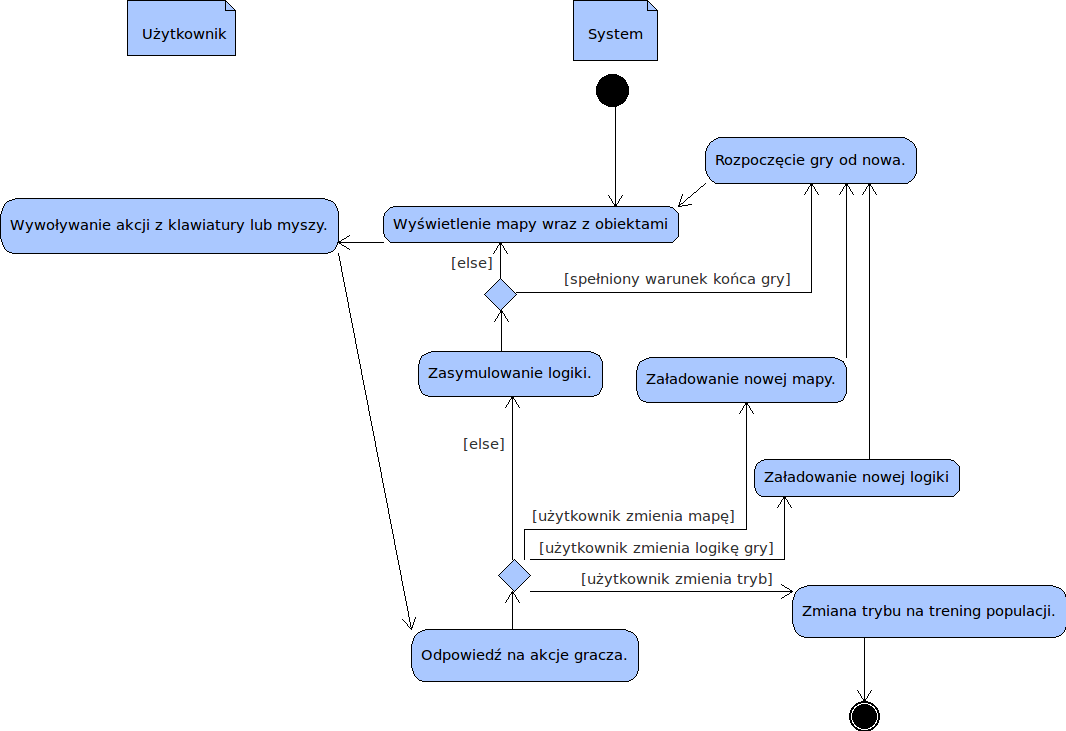
\includegraphics[width=\textwidth]{obrazki/activity_diagram.png}
		\caption{Diagram czynno�ci ``Przemieszczanie si� po mapie''.}
		\label{fig:activ1}
		\end{figure}
		\begin{figure}[!h]
		\centering
		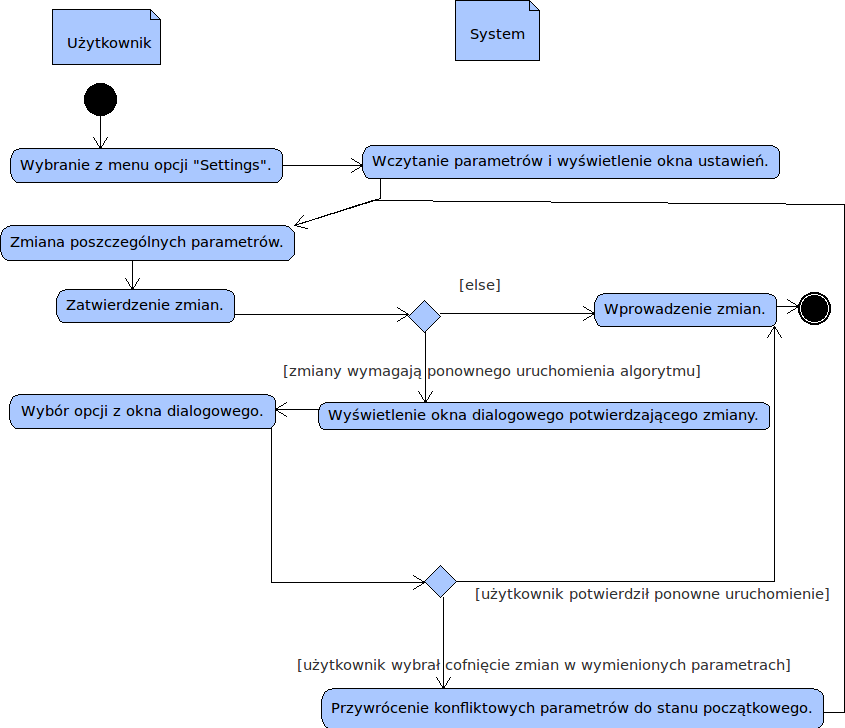
\includegraphics[width=\textwidth]{obrazki/activity_diagram_2.png}
		\caption{Diagram czynno�ci ``Zmiana ustawie� aplikacji''.}
		\label{fig:activ2}
		\end{figure}
		\FloatBarrier
\end{par}
\subsection{Diagram stan�w}
\begin{par}
	System sam w sobie nie posiada wielu stan�w jakie mo�e przyj��. Dwa g��wne stany to gra u�ytkownika w kt�rej akcje z klawiatury s� interpretowane jako ruchy gracza, oraz tryb treningu populacji.
	\begin{figure}[!h]
		\centering
		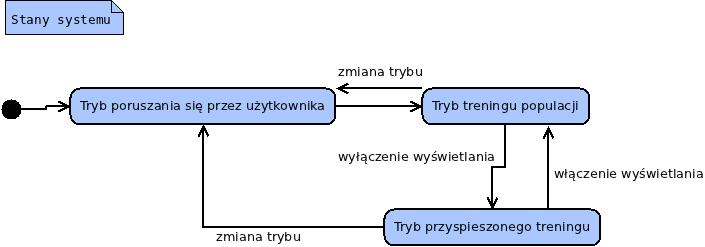
\includegraphics[width=\textwidth]{obrazki/diagram_stanow.jpg}
		\caption{Diagram czynno�ci ``Diagram stan�w systemu''.}
		\label{fig:stany}
		\end{figure}
	\FloatBarrier
	Stany dla Systemu (Rys. \ref{fig:stany}):
	U�ytkownik po uruchomieniu aplikacji mo�e porusza� si� postaci� po ekranie(stan ``Tryb poruszania si� przez u�ytkownika'').
	Je�li zmieni tryb dzia�ania systemu automatycznie przechodzi do trybu treningu (stan ``Tryb treningu populacji'').
	B�d�c w stanie treningu populacji u�ytkownik mo�e ponownie przej�� w tym swobodnego poruszania si�.
	U�ytkownik mo�e wy��czy� wy�wietlanie grafiki i tym samym przyspieszy� proces treningu (stan ``Tryb przyspieszonego treningu''). 
	Ze stanu treningu przyspieszonego u�ytkownik mo�e przej�� do trybu poruszania si� postaci� po ekranie poprzez zmian� trybu, b�d� do trybu treningu
	populacji poprzez w��czenie wy�wietlania grafiki.
\end{par}

\section{Modu� edytora map}
W tej cz�ci zostanie przedstawiona analiza wymaga� modu�u edytora map.
\subsection{Wymagania funkcjonalne}
	System nie wymaga r�nicowania u�ytkownik�w ze wzgl�du na role. Wymagania funkcjonalne wygl�daj� nast�puj�co:
	\begin{itemize}
		
		\item {\bf Otworzenie okna edytora map. }
		\newline
		Wa�nym elementem systemu jest narz�dzie pozwalaj�ce tworzy� nowe mapy oraz modyfikowa� istniej�ce.
		Powinno by� ono dost�pne jako osobne okno edytora map.
		\item {\bf Wczytywanie mapy do edytora. }
		\newline
		U�ytkownik powinien mie� mo�liwo�� edycji dowolnej wcze�niej stworzonej mapy, w tym celu powinien m�c z menu wybra� odpowiedni� opcj� pozwalaj�c� na wczytanie pliku mapy z dysku.
		Wczytywanie mo�e by� zrealizowane analogicznie do wczytywania mapy do �rodowiska gry.
		\item {\bf Zapis mapy do pliku. }
		\newline
		Podobnie jak odczyt, zapis mapy powinien by� dost�pny dla u�ytkownika z menu. 
		Dzi�ki zapisowi mapy na dysk twardy, u�ytkownik ma mo�liwo�� przechowywania wcze�niej tworzonych map, a co wa�niejsze otworzenie ich bezpo�rednio w symulatorze gry.
		\item {\bf Edycja mapy za pomoc� narz�dzi graficznych.}
		\newline
		Edycja mapy powinna by� intuicyjna i prosta nawet dla osoby nie znaj�cej szczeg��w formatu zapisu mapy. 
		Poniewa� ka�dy obiekt w grze posiada prostok�tny obszar kolizji, edytor powinien pozwala� na �atwe tworzenie prostok�tnych obiekt�w.
		Zrealizowane mo�e by� to przez wyznaczanie dw�ch rog�w prostok�ta za pomoc� metody ``przeci�gnij i upu��''.
		Narz�dzia powinny by� dost�pne po wybraniu odpowiedniej ikony w panelu narz�dzi edytora map.
		Przydatne w edycji map mog� okaza� si� cz�sto u�ywane akcje takie jak cofni�cie ostatniej zmiany, zaznaczenie element�w w edytorze i usuwanie ich, b�d� czyszczenie ca�ej mapy.
	\end{itemize}
\subsection{Wymagania niefunkcjonalne}
	\begin{itemize}
	\item {\bf Otwarty format mapy. }	
	\newline
	Istotn� rzecz� mo�e by� tutaj przechowywanie mapy w pliku tekstowym. 
	O ile zapis binarny mo�e okaza� si� szybszy i bardziej kompaktowy, to wa�niejsze jest jednak
	umo�liwienie u�ytkownikom edycji mapy r�cznie, b�d� poprzez programy trzecie. Dzi�ki temu mo�liwe b�dzie generowanie np. bardzo d�ugich losowych map.
	\end{itemize}


\subsection{Diagram przypadk�w u�ycia}
\begin{par}
	Diagram przypadk�w u�ycia zosta� przedstawiony na Rys. \ref{fig:diagram_przypadkow_mapa}.
		\begin{figure}[!h]
		\centering
		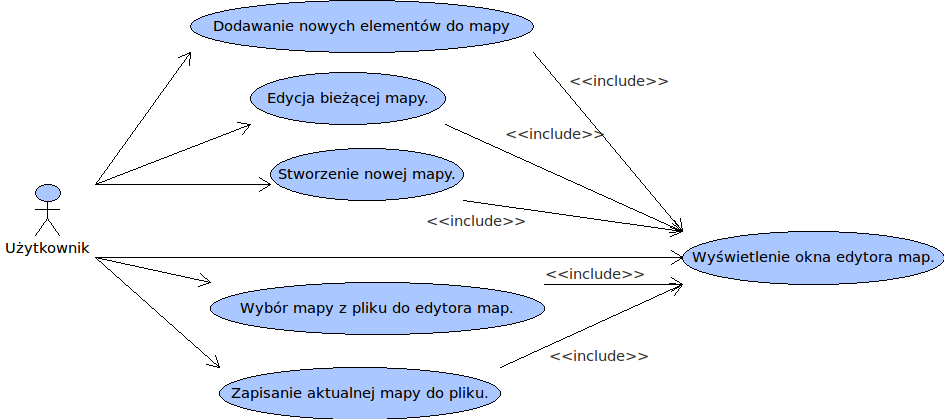
\includegraphics[width=\textwidth]{obrazki/use_case_editor.png}
		\caption{Diagram przypadk�w u�ycia modu�u edytora map.}
		\label{fig:diagram_przypadkow_mapa}
		\end{figure}
		\FloatBarrier
\end{par}
\subsection{Opis tekstowy przypadk�w u�ycia}
\begin{par}
	We wszystkich przypadkach u�ycia aktorem jest u�ytkownik aplikacji.
	\begin{itemize}

	\item
	Opis przypadku u�ycia {\bf Edycja bie��cej mapy. }.
	\begin{enumerate}
	\item Podstawowy ci�g zdarze�:
		\begin{enumerate}
		\item U�ytkownik klika w przycisk menu dotycz�cy edytora map.
		\item Wy�wietlone zostaje nowe okno aplikacji zawieraj�ce przyciski dotycz�ce edycji mapy.
		\item Do edytora map domy�lnie zostaje wczytana bie��ca mapa wczytana do �rodowiska symulatora.
		\item U�ytkownik wybiera obiekty gry u�yciu przycisk�w znajduj�cych si� w menu okna a nast�pnie metod� przeci�gnij-upu�� rysuje prostok�tne obiekty odpowiadaj�ce za obiekty w grze.
		\item U�ytkownik z menu wybiera opcj� zapisu mapy do pliku.
		\item Wy�wietlone zostaje okno dialogowe zapisu pliku w kt�rym u�ytkownik wybiera nazw� pliku.
		\item U�ytkownik zamyka okno edytora map.
		\end{enumerate}
	\item Alternatywne ci�g zdarze�:
		\begin{enumerate}
		\item U�ytkownik wczytuje nowa map� do edytora map. 
			\begin{enumerate}
			\item Wy�wietlone zostaje okno dialogowe dotycz�ce otwarcia pliku z systemu.
			\item Wszystkie obiekty z planszy zostaj� usuni�te, i wczytywane s� nowe z wybranej wcze�niej mapy.
			\end{enumerate}
		\end{enumerate}
	\item Zale�no�ci czasowe:
		\begin{enumerate}
		\item Cz�stotliwo�� wykonania: 0-5 razy w ci�gu dzia�ania aplikacji.
		\item Typowy czas realizacji: 5 minut.
		\item Maksymalny czas realizacji: nieokre�lony.
		\end{enumerate}
	\item Warto�ci uzyskiwane przez aktor�w po zako�czeniu przypadku u�ycia:
		\begin{enumerate}
		\item U�ytkownik po zapisaniu stworzonej mapy do pliku ma mo�liwo�� wczytania mapy z dysku do symulatora gry i przeprowadzenia treningu populacji na nowej mapie.
		\end{enumerate}
	\end{enumerate}

	\item
	Opis przypadku u�ycia {\bf Stworzenie nowej mapy. }.
	\begin{enumerate}
	\item Podstawowy ci�g zdarze�:
		\begin{enumerate}
		\item U�ytkownik wybiera z menu przycisk dotycz�cy edytora map.
		\item Do edytora map domy�lnie zostaje wczytana bie��ca mapa wczytana do �rodowiska symulatora.
		\item U�ytkownik z panelu narz�dzi edytora map wybiera usuni�cie wszystkich obiekt�w z mapy.
		\item System usuwa obiekty z edytora map.
		\item U�ytkownik za pomoc� narz�dzi buduje elementy nowej mapy.
		\item U�ytkownik z menu wybiera opcj� zapisu mapy do pliku.
		\item Wy�wietlone zostaje okno dialogowe zapisu pliku w kt�rym u�ytkownik wybiera nazw� pliku.
		\item U�ytkownik zamyka okno edytora map.
		\end{enumerate}
	\item Zale�no�ci czasowe:
		\begin{enumerate}
		\item Cz�stotliwo�� wykonania: 0-5 razy w ci�gu dzia�ania aplikacji.
		\item Typowy czas realizacji: 5 minut.
		\item Maksymalny czas realizacji: nieokre�lony.
		\end{enumerate}
	\item Warto�ci uzyskiwane przez aktor�w po zako�czeniu przypadku u�ycia:
		\begin{enumerate}
		\item U�ytkownik po utworzeniu nowej mapy ma mo�liwo�� wczytania jej w symulatorze.
		\end{enumerate}
	\end{enumerate}
	\end{itemize}
\end{par}

\subsection{Diagramy czynno�ci}
\begin{par}
		Poni�ej zostan� przedstawione diagramy najistotniejszych czynno�ci w systemie dotycz�ce modu�u edytora map.
		\begin{figure}[!h]
		\centering
		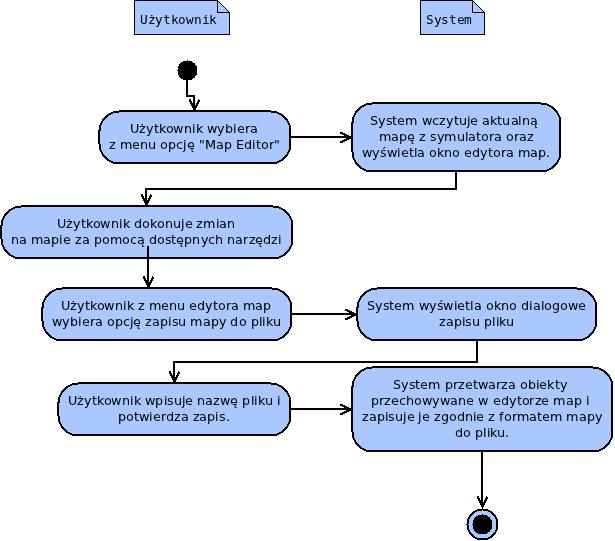
\includegraphics[width=\textwidth]{obrazki/czynnosci_edytor_map.jpeg}
		\caption{Diagram czynno�ci ``Edycja bie��cej mapy''.}
		\label{fig:czynn_edytor_map}
		\end{figure}
		\FloatBarrier
\end{par}



\section{Diagram klas}
\begin{par}
	\begin{par}
	Diagram klas projektu przedstawiony zosta� na rysunku \ref{fig:diagram_klas}.
	\end{par}
	\begin{figure}[!h]
	\centering
	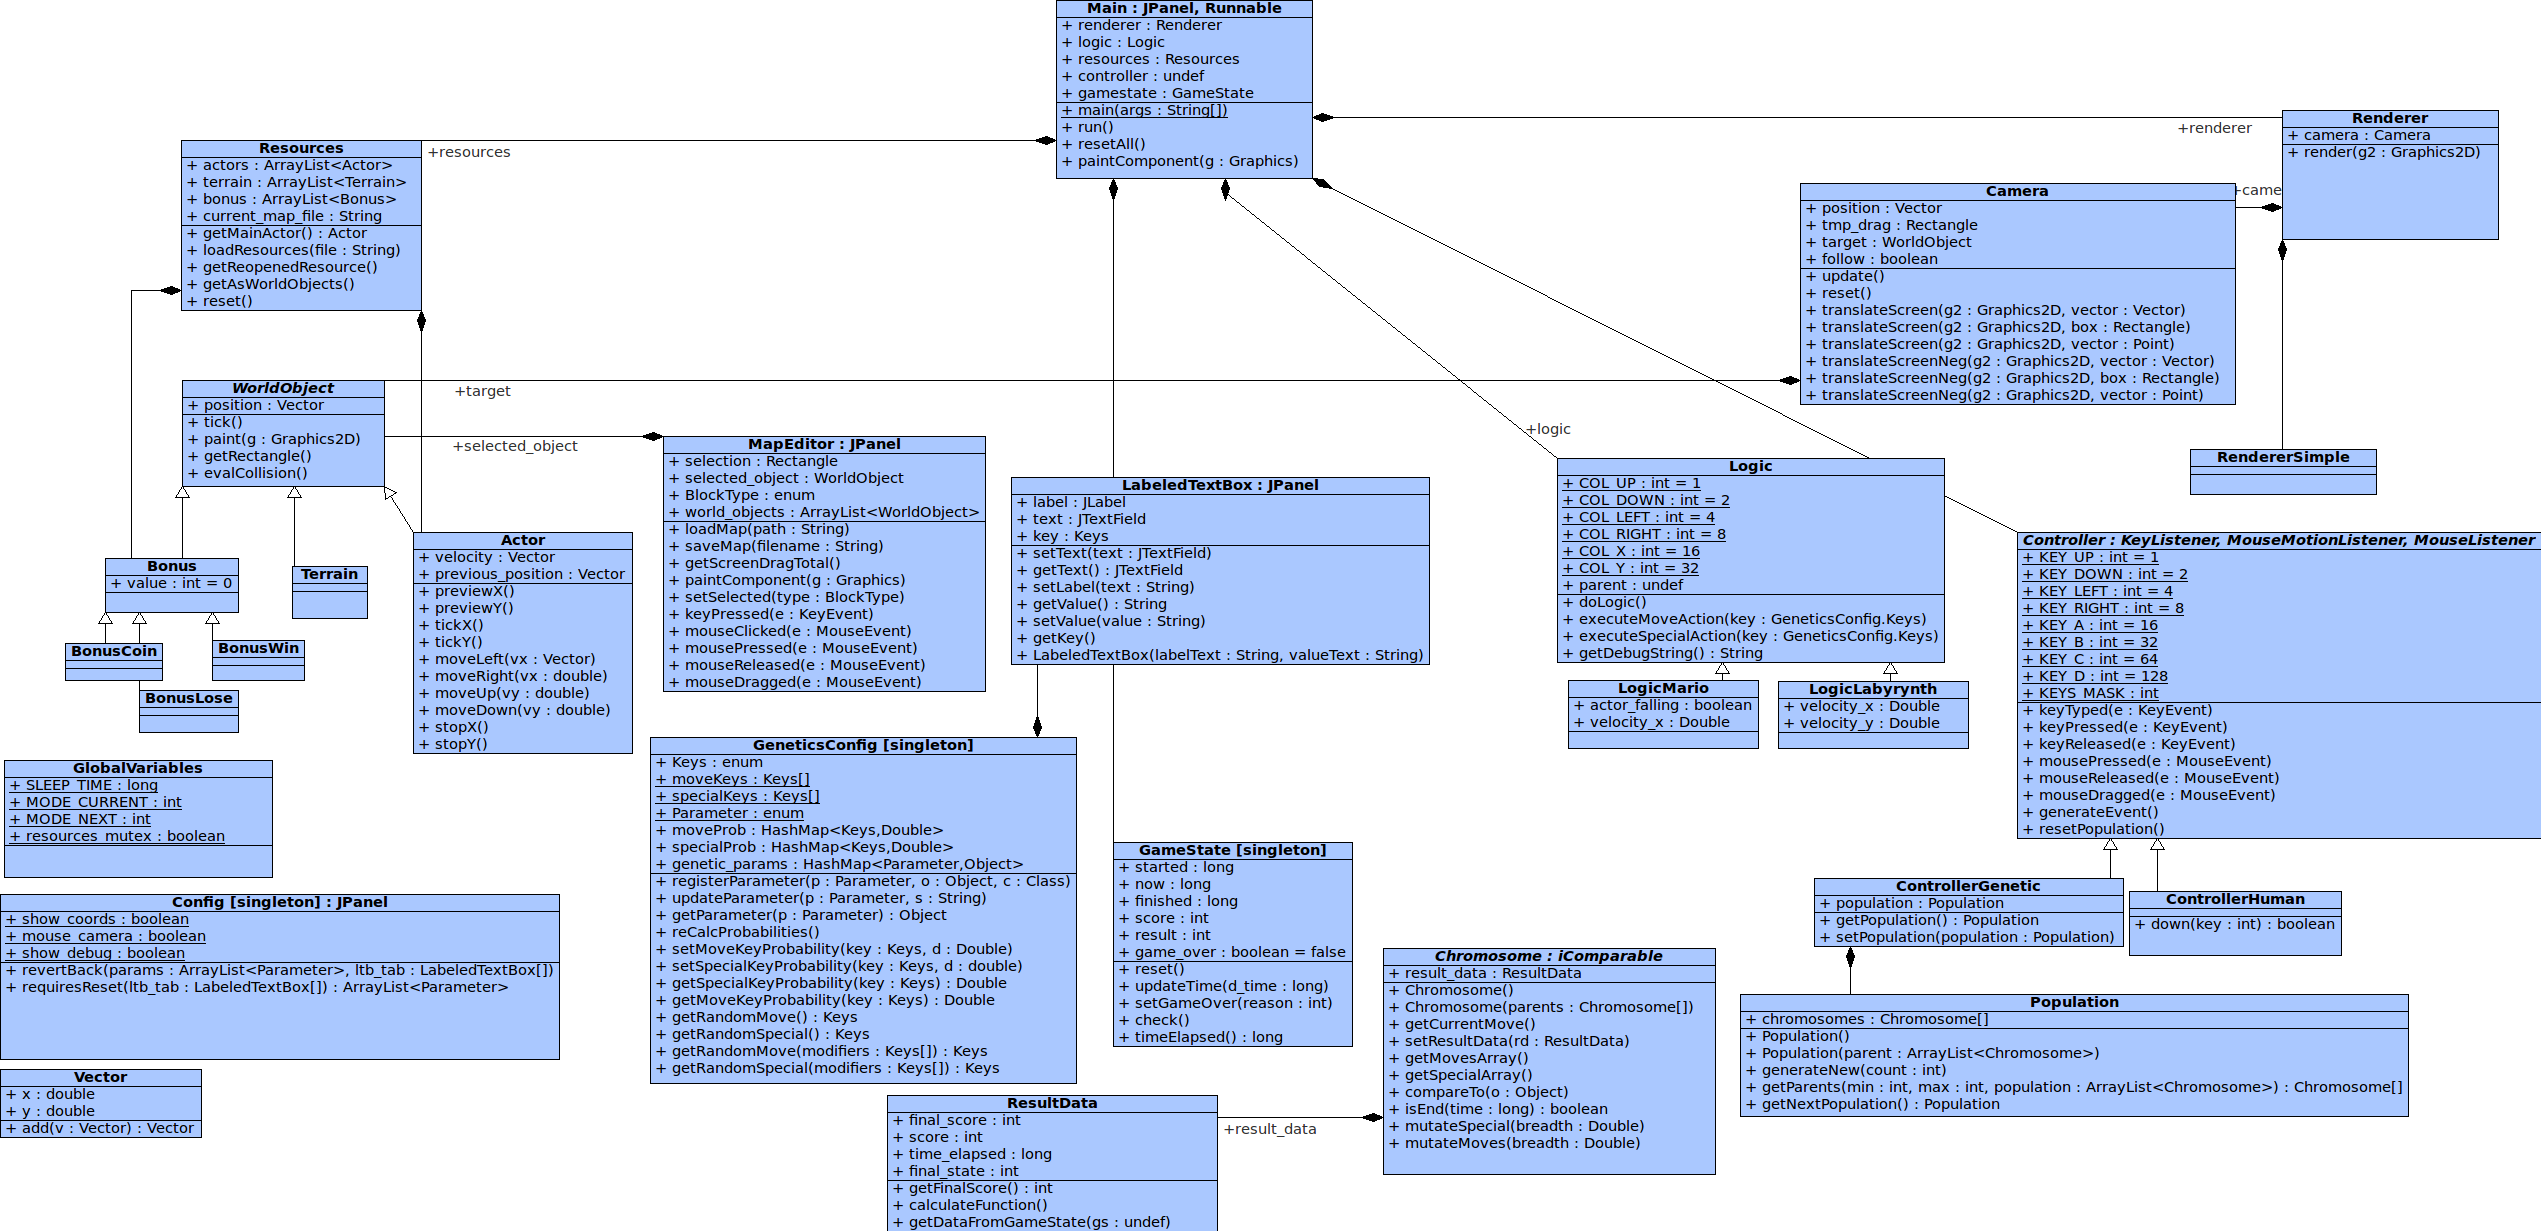
\includegraphics[height=\textheight]{obrazki/diagram_klas.png}
	\caption{Diagram Klas.}
	\label{fig:diagram_klas}
	\end{figure}
	Poni�ej zosta�y opisane poszczeg�lne klasy w kolejno�ci alfabetycznej.
	\begin{enumerate}
	\item{\bf Actor }\newline
	Actor jest klas� dziedzicz�c� po klasie WorldObject. Reprezentuje ona obiekt postaci poruszaj�cej si� po ekranie w �rodowisku gry. Poniewa� instancja obiektu Actor jest przemieszczaj�cym si� obiektem niezb�dne by�o dodanie wektora pr�dko�ci do klasy, kt�ry odpowiada za zmian� pozycji w czasie. Klasa posiada metody takie jak moveLeft, moveRight, moveUp oraz moveDown pozwalaj�ce na �atw� zmian� kierunku ruchu aktora. Metody tickX, tickY aktualizuj� pozycje gracza. Aby wykry� kolizj� mo�liwe jest wywo�anie metody previewX (odp. previewY) kt�ra zwraca ``przysz��'' pozycj� obiektu po wykonaniu przez niego ruchu w osi X (odp. osi Y).
	\item{\bf Bonus }\newline
	Klasa Bonus jest abstrakcyjn� klas� dziedzicz�c� po klasie WorldObject. Odpowiada ona za obiekty wp�ywaj�ce na przebieg gry. Kolizja aktora z obiektem powoduje wywo�anie metody evalCollision, kt�ra decyduje o efekcie zdarzenia. Obiekty Bonus posiadaj� przypisan� warto�� punktow� kt�ra w zale�no�ci od typu obiektu r�nie wp�ywa na rozgrywk�.
	\item{\bf BonusCoin }\newline
	Klasa BonusCoin reprezentuje jedynie punkty umieszczone na planszy. Kolizja z obiektem klasy BonusCoin powoduje zwi�kszenie licznika punk�w gracza b�d� osobnika populacji. Poza dodaniem punkt�w obiekt klasy BonusCoin nie wp�ywa bezpo�rednio na przebieg gry.
	\item{\bf BonusLose }\newline
	Obiekt klasy BonusLose reprezentuje obiekt ko�cz�cy gr� ze skutkiem negatywnym. Kolizja aktora z obiektem automatycznie ko�czy przebieg gry ze skutkiem RESULT\_LOST.
	\item{\bf BonusWin }\newline
	Obiekt klasy BonusWin stanowi cel ka�dej gry. Kolizja z obiektem typu BonusWin automatycznie ko�czy rozgrywk� ze skutkiem RESULT\_WON, co jest brane pod uwag� podczas liczenia funkcji przystosowania.
	\item{\bf Camera }\newline
	Obiekt Camera przechowuje wektor przesuni�cia obrazu i jest u�ywany do przesuwania ekranu. Jest on wykorzystywany podczas symulacji do ``pod��ania'' za obiektem gracza, b�d� do swobodnego przesuwania ekranu gry za pomoc� myszy. Analogicznie w edytorze map u�ytkownik ma mo�liwo�� przesuwania ekranu za pomoc� myszy, co upraszcza tworzenie du�ych map. Obiekt Camera przechowuje r�wnie� referencj� do aktualnie �ledzonego obiektu.
	Metoda update pozwala na aktualizowanie kamery wraz z przesuwaniem si� postaci po ekranie.
	metody translateScreen oraz translateScreenNeg odpowiednio przesuwaj� ekran o ��dany wektor przesuni�cia.
	\item{\bf Config }\newline
	Klasa Config przechowuje zmienne dotycz�ce konfiguracji programu, wykorzystywane w celu wyszukiwania b��d�w. Przechowuje ona ustawienia wy�wietlania informacji o pozycji ka�dego obiektu w grze, b�d� dodatkowych zmiennych takich jak czas kt�ry up�yn�� od pocz�tku gry.
	Domy�lnie informacje te nie s� widoczne, lecz mo�na je w��czy� z panelu konfiguracyjnego.
	Opr�cz tego klasa Config dziedziczy po klasie JPanel, i stanowi g��wny element panelu konfiguracyjnego programu.
	\item{\bf Controller }\newline
	Klasa Controller jest klas� po�rednicz�c� w wymianie informacji pomi�dzy sygna�ami z klawiatury, b�d� akcjami zapisanymi w chromosomie, a �rodowiskiem gry. Odseparowuje ona obie warstwy dzi�ki czemu mo�liwe jest pisanie logiki gry, b�d� reakcji na poszczeg�lne akcje, niezale�nie od �r�d�a sygna�u. Klasa Controller jest klas� abstrakcyjn� i uzupe�nia interfejsy takie jak KeyListener, MouseListener, MouseMotionListener (tym samym implementuje wszystkie zwi�zane z nimi metody), dzi�ki czemu wszelkie zdarzenia wywo�ane w oknie gry zostaj� przechwycone i odpowiednio obs�u�one. Klasa Controller posiada r�wnie� zmienne ca�kowite kt�re s� kolejnymi pot�gami 2, zwi�zane jest to z optymalizacj� przechwytywania ruch�w z klawiatury - ka�de wci�ni�cie klawisza ustawia odpowiedni bit.
	\item{\bf ControllerHuman }\newline
	Klasa dziedzicz�ca po klasie Controller, nadpisuje powy�sze metody, tak aby wci�ni�cia klawiszy przez gracza odpowiednio porusza�y postaci� w grze. Posiada ona metod� down(int) kt�ra zwi�zana jest z wy�ej wymienion� optymalizacj� przechwytywania ruchu. Dzi�ki operacjom bitowym szybko sprawdzany jest stan ka�dego klawisza.
	\item{\bf ControllerGenetic }\newline
	Klasa dziedzicz�ca po klasie Controller, odpowiada za odczytywanie wygenerowanych akcji z osobnik�w znajduj�cych si� w populacji i odpowiednie przekazywanie ich do �rodowiska gry (logiki). Instancja klasy zawiera w sobie obiekt klasy Population kt�ry przechowuje ca�� populacj� osobnik�w.
	\item{\bf Chromosome }\newline
	Chromosome jest klas� reprezentuj�c� obiekt osobnika. Uzupe�nia ona interfejs Comparable, dzi�ki czemu mo�liwe jest wykorzystanie algorytm�w sortuj�cych ze standardowej biblioteki javy. Ka�dy obiekt tej klasy zawiera w sobie instancje obiektu ResultData kt�ra przechowuje dane na temat wyniku gry. Klasa posiada metody takie jak mutateSpecial i mutateMoves kt�re odpowiednio dokonuj� mutacji osobnika na tablicy akcji specjalnych i tablicy ruch�w. Parametr breadth decyduje o ``rozleg�o�ci'' mutacji, np: warto�� 0.2 spowoduje mutacj� losowych 20\% akcji w danej tablicy chromosomu. Opr�cz standardowego konstruktora klasy jest tak�e konstruktor przyjmuj�cy tablic� innych chromosom�w. Traktowane jest to jako tworzenie nowego Chromosomu na podstawie kilku innych, czyli opisane wcze�niej krzy�owanie statystyczne z grupy rodzicielskiej z poprzedniej populacji. 
	\item{\bf GameState }\newline
	Klasa GameState przechowuje aktualny stan gry, wraz ze zmiennymi takimi jak: czasy rozpocz�cia gry, czas aktualny oraz czas zako�czenia (wszystkie warto�ci jako czasy systemowe w milisekundach), zebrane przez posta� punkty oraz warto�� wyliczona z funkcji przystosowania. Funkcja updateTime(d\_time) aktualizuje czas gry na podstawie faktycznego czasu kt�ry up�yn�� w systemie, dzi�ki czemu gra z punktu widzenia logiki przebiega tak samo bez wzgl�du na wydajno�� komputera na kt�rym uruchamiany jest program.
	\item{\bf GeneticsConfig }\newline
	Klasa GeneticsConfig przechowuje wszystkie informacje dotycz�ce parametr�w algorytmu genetycznego. Warto�ci prawdopodobie�stw wylosowania akcji specjalnych (specialProb) b�d� ruchu postaci (moveProb) przechowywane s� w strukturach typu HashMap dost�pnych w standardowych bibliotekach javy.
	Opr�cz prawdopodobie�stw klasa przechowuje te� parametry algorytm�w genetycznych takie jak rozmiar populacji, wielko�� tablicy chromosomu, sta�� krzy�owania, czy rozleg�o�� mutacji poszczeg�lnych tablic. Parametry te r�wnie� przechowywane s� w tablicy asocjacyjnej, dzi�ki czemu mo�liwe jest odwo�ywanie si� do nich poprzez typ wyliczeniowy ``Parameter''.
	Opr�cz samych warto�ci przechowywany jest te� typ ka�dego parametru. Metody registerParameter, updateParameter oraz getParameter s�u�� do aktualizacji b�d� pobierania parametr�w z tablicy. Klasa opr�cz przechowywania warto�ci posiada metody zwracaj�ce losowy ruch. Korzysta z tego g��wnie klasa Chromosome przy generowaniu nowych osobnik�w.
	\item{\bf GlobalVariables }\newline
	Klasa GlobalVariables przechowuje zmienne statyczne widoczne w ca�ym systemie takie jak aktualny tryb pracy, zmienn� SLEEP\_TIME decyduj�c� o tempie gry oraz zmienn� odpowiadaj�c� za zablokowywanie dost�pu do zasob�w - program jako aplikacja okienkowa korzysta z dw�ch w�tk�w wobec czego jest to koniecznie przy wsp�dzieleniu zasob�w takich jak obiekty gry.
	\item{\bf LabeledTextBox }\newline
	Jest to klasa pomocnicza przy tworzeniu interfejsu u�ytkownika - dzi�ki niej mo�liwe jest automatycznie generowanie par JLabel i JTextBox widocznych w oknie ustawie� aplikacji.
	\item{\bf Logic }\newline
	Klasa Logic odpowiada za symulacj� logiki gry - g��wnie dotyczy to aktora i jego reakcji na r�nego rodzaju akcje, gdy� jest on jedynym ruchomym obiektem w grze. Dzi�ki odseparowaniu logiki gry od pozosta�ych warstw mo�liwe jest proste rozszerzanie systemu o w�asne regu�y gry. Klasa posiada metod� doLogic kt�ra jest cyklicznie wykonywana w ka�dej p�tli gry. Opr�cz tego metody executeMoveAction oraz executeSpecialAction decyduj� o reakcji �rodowiska oraz aktora na akcje generowane przez chromosom, b�d� u�ytkownika.
	\item{\bf LogicLabirynth }\newline
	Jest to przyk�adowa implementacja gry, w kt�rej posta� mo�e porusza� si� w 4 kierunkach. 
	G��wnym za�o�eniem logiki ma by� realizacja gier rozwi�zujacych dwuwymiarowy labirynt.
	Klasa zosta�a rozszerzona o warto�ci ruchu postaci w obu osiach.
	\item{\bf LogicMario }\newline
	Podobnie jak klasa LogicLabirynth jest to prosta implementacja gry wzorowanej na grze Super Mario Brothers. Pomocnicza zmienne actor\_falling pomaga w realizacji fizyki w grze (wp�ywie grawitacji na posta�). Zmienna velocity\_x odpowiada za warto�� pr�dko�ci postaci w poziomie.
	\item{\bf Main }\newline
	Klasa Main jest g��wn� klas� w systemie. Zawiera ona referencje do poszczeg�lnych komponent�w systemu takich jak silnik renderuj�cy, logika gry, mapy gry, warstwy kontroluj�cej wykonywanie akcji oraz bie��cego stanu gry.
	Podczas uruchomienia aplikacji uruchamiana jest metoda main(String[]) kt�ra inicjuje wszystkie koniecznie komponenty i wy�wietla okno aplikacji.
	Klasa uzupe�nia interfejs Runnable, dzi�ki czemu dzia�a jako osobny w�tek. Oprocz tego klasa Main dziedziczy po klasie JPanel i nadpisuje metod� painComponent(Graphics), dzi�ki czemu mo�liwe jest stworzenie warstwy wizualizacyjnej dla �rodowiska gry.
	\item{\bf MapEditor }\newline
	Klasa MapEditor podobnie jak klasa Main dziedziczy po klasie JPanel. Zawiera ona list� obiekt�w niezale�n� od obiekt�w istniej�cych w symulatorze gry. Metoda loadMap pozwala na wczytanie mapy z pliku na dysku, metoda saveMap s�u�y do zapisu aktualnie edytowanej mapy do pliku tekstowego. Klasa uzupe�nia interfejsy MouseListener oraz MouseMotionListener przez co nadpisuje metody s�u��ce do obs�ugi zdarze�. 
	\item{\bf Population }\newline
	Klasa Population przechowuje tablic� osobnik�w bior�cych udzia� w treningu populacji. 
	Metoda getNextPopulation odpowiada za wygenerowanie nowej populacji na podstawie wynik�w poprzedniej - to w niej wykonywane s� wszystkie kroki zwi�zane z algorytmem genetycznym.
	Opr�cz tego klasa posiada konstruktor generuj�cy now� Populacj� na podstawie populacji rodzicielskiej (wspomniane wcze�niej krzy�owanie statystyczne). Metoda getParents zwraca populacj� rodzicielsk� na podstawie aktualnej populacji.
	\item{\bf Renderer }\newline
	Renderer jest klas� odpowiedzialn� za wy�wietlanie element�w gry w oknie. Warstwa ta zosta�a odseparowana, dzi�ki czemu podczas dalszej rozbudowy aplikacji �atwo mo�na zast�pi� silnik renderuj�cy na inny, b�d� wprowadzi� u�ywanie tekstur do programu.
	\item{\bf RendererSimple }\newline
	Jest to prosta implementacja silnika renderuj�cego. G��wnym za�o�eniem jest tutaj jedynie rysowanie prostok�tnych obiekt�w, r�ni�cych si� kolorami (Ka�da klasa dziedzicz�ca po WorldObject posiada inny kolor).
	\item{\bf Resources }\newline
	Klasa Resources przechowuje wszystkie obiekty �wiata gry. Metoda loadResources(String) interpretuje plik tekstowy przekazany w parametrze jako �cie�ka na dysku i zamienia opis tekstowy mapy na obiekty w grze. Warto zauwa�y� i� metoda getMainActor zwraca jeden obiekt Aktora, natomiast w zasobach gry mo�e by� ich kilku (kolekcja actors jest list�). Jest to rozwi�zanie maj�ce na celu p�niejsze rozwini�cie systemu np. do obs�ugi gry wieloosobowej.
	\item{\bf ResultData }\newline
	ResultData jest klas� pomocnicz� przechowuj�c� dane na temat przej�cia gry ka�dego osobnika. Przechowuje ona zmienne takie jak wynik funkcji przystosowania (zmienna final\_score), ilo�� zebranych punkt�w na mapie (score), czas przej�cia (time\_elapsed) oraz stan w jakim przej�cie si� zako�czy�o (final\_state przyjmuj�cy warto�ci RESULT\_TIMEOUT, RESULT\_WON b�d� RESULT\_LOST). Opr�cz tego posiada ona metod� licz�c� funkcj� przystosowania na podstawie parametr�w w ustawieniach algorytmu genetycznego.
	\item{\bf Terrain }\newline
	Klasa Terrain jest klas� dziedzicz�c� po klasie WorldObject. Odpowiada za statyczny teren. Najcz�ciej kolizja z nim powoduje zatrzymanie ruchu, jednak zale�y to od implementacji logiki gry.
	\item{\bf Vector }\newline
	Klasa pomocnicza przechowuj�ca wsp�rz�dne punktu (typ double).
	\item{\bf WorldObject }\newline
	Klasa abstrakcyjna po kt�rej dziedzicz� wszystkie elementy gry. Podstawow� jej zmienn� jest po�o�enie na mapie oraz rozmiar (odpowiednio zmienne ``position'' oraz ``size'').
	Klasa posiada metod� getRectangle zwracaj�c� obiekt Rectangle dost�pny w standardowej bibliotece, dzi�ki czemu realizowanie kolizji pomi�dzy dwoma obiektami jest realizowanie poprzez wywo�anie metody intersects(Rectangle). Ka�dy dziedzicz�cy po WorldObject obiekt ma do dyspozycji metod� evalCollision kt�ra decyduje o czynno�ciach wykonywanych podczas kolizji dw�ch obiekt�w. Obiekty klasy WorldObject posiadaj� r�wnie� metod� paint(Graphics) kt�ra odpowiada za rysowanie obiektu na ekranie (obiekcie Graphics).
	\end{enumerate}

\end{par}



\chapter{Opis interfejsu systemu}
\section{Modu� silnika i symulatora gry}
\subsection{G��wne okno aplikacji}
\begin{par}
Podstawowym oknem aplikacji widocznym tu� po uruchomieniu jest g��wne okno symulatora gry. 
Domy�lnym trybem jest tryb poruszania si� po mapie przez u�ytkownika. 
\begin{itemize}
\item Sterowanie postaci� przez klawiatur� zrealizowanie jest za pomoc� strza�ek kierunkowych, oraz klawiszy $a,s,d,f$ jako akcji specjalnych.
\item Reakcja �rodowiska na poszczeg�lne klawisze zale�y od logiki gry. 
\item Domy�ln� logik� w systemie jest instancja klasy LogicMario: strza�ki kierunkowe odpowiadaj� za ruch postaci (tylko w osi poziomej), natomiast klawisz f odpowiada za skok postaci.
\item Logika LogicLabirynth zak�ada ruch postaci w 4 kierunkach, bez wp�ywu innych si� na posta� (takich jak grawitacja). Akcje specjalne nie s� wykorzystywane.
\end{itemize}
\begin{par}
	Poniewa� dzia�anie algorytmu nie jest zwi�zane z fizyk� ani zasadami obowi�zuj�cymi w grze, system mo�e dzia�a� dla wielu r�nych typ�w gier platformowych i zr�czno�ciowych.
	Jedynym wymogiem jest to i� musz� one da� si� opisa� za pomoc� wy�ej zdefiniowanych klas i cech:
	\begin{enumerate}
		\item
			Obiekty �wiata musz� nale�e� do kt�rej� z klas dziedzicz�cych po klasie \textit{WorldObject}.
		\item 
			Mo�liwe rezultaty zako�czenia algorytmu musz� by� w�r�d zbioru rezultat�w: \{Koniec Czasu, Wygrana, Przegrana\}, 
		\item
			Rodzaje mo�liwych akcji do wykonania w grze musz� by� przypisane do 4 akcji ruchu kierunkowego oraz 4 akcji specjalnych.
	\end{enumerate}
	Jedyn� prac� jak� nale�y wykona� przy implementacji w�asnego �rodowiska gry jest uzupe�nienie w�asnej klasy dziedzicz�cej po klasie \textit{Logic}.
	W�wczas przy poprawnej implementacji logiki gry system automatycznie symuluje zbiory chromosom�w w �rodowisku gry.
\end{par}
Poni�ej przedstawiony zosta� opis poszczeg�lnych element�w g��wnego okna aplikacji.
\begin{figure}[!h]
		\centering
		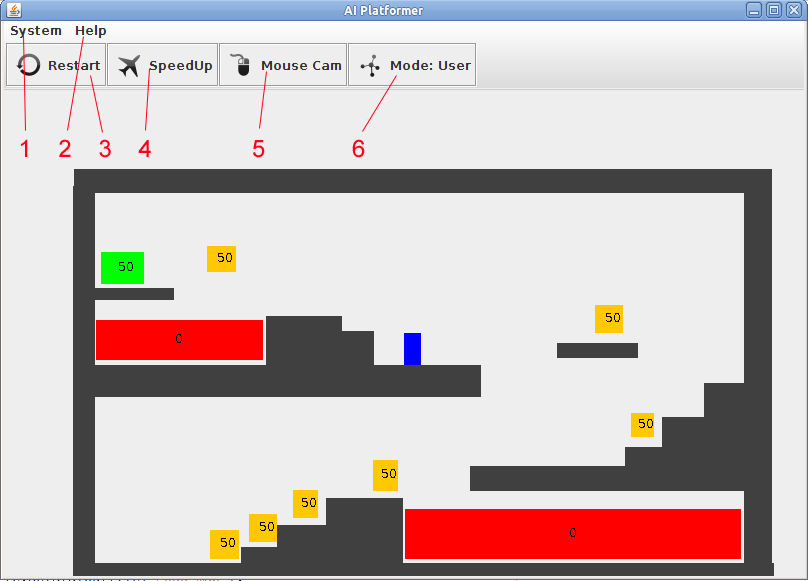
\includegraphics[width=4in]{obrazki/main_window.png}
		\caption{G��wne okno aplikacji.}
		\label{fig:main_window}
	\end{figure}
W oknie aplikacji widoczne jest menu oraz pasek narz�dzi zawieraj�cy podstawowe przyciski steruj�ce systemem:
	\begin{enumerate}
	\item Z menu ``System'' u�ytkownik ma mo�liwo�� otwarcia dodatkowych okien aplikacji takich jak edytor map, panel ustawie�, podgl�d populacji oraz menu dialogowe dotycz�ce wczytania nowej mapy z pliku do �rodowiska gry.
	\item Menu ``Help'' zawiera informacje dotycz�ce programu oraz kr�tki opis skr�t�w klawiszowych.
	\item Przycisk ``Restart'' pozwala na ponowne uruchomienie algorytmu, czyli wygenerowanie losowej populacji.
	\item Przycisk ``SpeedUp'' odpowiada za przej�cie systemu w tryb treningu przyspieszonego, je�li populacja aktualnie znajduje si� w trybie treningu. Przestaje w�wczas by� aktualizowana grafika, a system w tle symuluje kolejne populacje osobnik�w w �rodowisku gry.
	\item Domy�lnym trybem kamery jest �ledzenie obiektu aktora. Przycisk ``Mouse Cam'' pozwala na przej�cie w tryb swobodnej kamery - prawy przycisk myszy s�u�y do ``przesuwania'' ekranu.
	\item Przycisk ``Mode: User''(``Mode: Genetic'') s�u�y do zmiany trybu dzia�ania systemu. Domy�lnie pierwszym trybem jest tryb poruszania si� po mapie przez u�ytkownika. Po wci�ni�ciu przycisku system przechodzi do trybu treningu populacji. Kolejne wci�ni�cie przycisku przywraca poprzedni tryb swobodnego poruszania si�.
	\end{enumerate}
	\FloatBarrier
\end{par}
\begin{par}
	�rodowisko gry znajduje si� w centralnej cz�ci okna gry.
	Wszystkie elementy gry z punktu widzenia kolizji s� prostok�tnymi obszarami, r�ni�cymi si� reakcj� na kolizj� z obiektem gracza. W podstawowym silniku renderuj�cym zosta�y one wyr�nione kolorem.
	
	\definecolor{orange}{rgb}{1,0.5,0}
	\definecolor{gray}{rgb}{0.5,0.5,0.5}
	Na Rys. \ref{fig:objects} wida� obiekty �wiata gry: 
	\textcolor{blue}{\textit{Actor}}, 
	\textcolor{orange}{\textit{BonusCoin}},
	\textcolor{red}{\textit{BonusLose}},
	\textcolor{green}{\textit{BonusWin}},
	\textcolor{black}{\textit{Terrain}}.

	\begin{figure}[!h]
		\centering
		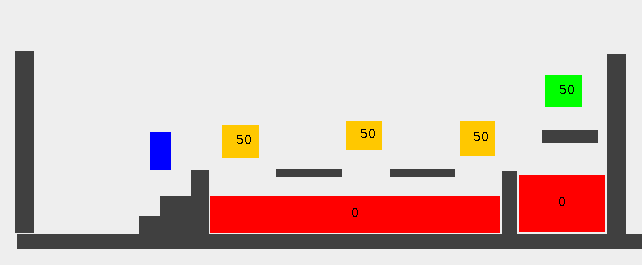
\includegraphics[width=4in]{obrazki/objects.png}
		\caption{Poszczeg�lne obiekty �wiata gry.}
		\label{fig:objects}
	\end{figure}
\end{par}
\subsection{Panel konfiguracyjny}
\begin{par}
	Jak ju� zosta�o wspomniane, podstaw� dobrego systemu, szczeg�lnie do zastosowa� badawczych jest �atwo dost�pna konfiguracja. 
	W pracy rol� t� pe�ni po�rednio klasa \textit{GeneticsConfig} kt�ra zawiera wszystkie najwa�niejsze parametry dotycz�ce algorytmu. S� przechowywane jako warto�ci tablicy asocjacyjnej (klasa \textit{HashMap}). 
	Opr�cz tego sama tablica zosta�a opakowana w taki spos�b i� rejestracja nowej warto�ci do tablicy wi��e si� z automatycznym wygenerowaniem odpowiedniego pola w panelu konfiguracyjnym - dzi�ki temu dodanie kolejnych parametr�w genetycznych przy przysz�ym rozbudowywaniu aplikacji automatycznie aktualizuje panel konfiguracyjny.
\end{par}
\begin{par}
	Ka�da z akcji, zar�wno ruchu jak i tablica akcji specjalnych posiada pewne prawdopodobie�stwo wyst�pienia.
	Zosta�y one podzielone na dwie grupy: \textit{Movement key probabilities} oraz \textit{Special key probabilities}
	Warto�ci te mo�liwe s� do zmiany w panelu konfiguracyjnym, przy czym s� one normalizowane do sumy wszystkich warto�ci z danej kategorii.
	Przyk�adowo dla warto�ci podanych na rys \ref{fig:config1}. Warto�� ruchu w prawo (grupa ``Movement key probabilities'') wynosi $\frac{0.7}{0.7+0.4}=0.6364$.
	Aby nie bra� pod uwag� akcji kt�re i tak nie b�d� interpretowane przez logik�, najlepiej jest ustawi� prawdopodobie�stwo wylosowania ruch�w nieaktywnych na warto�� $0$. 
	Mapa gry mo�e by� ukierunkowana b�d� nie, w�wczas ustawienie odpowiedniego stosunku akcji ruchu mo�e znacznie przyspieszy� znalezienie wyniku. Przyk�adowo: Je�li problemem jest znalezienie rozwi�zania na szerokiej mapie, kt�rej cel znajduje si� w jej prawym kra�cu, dobr� strategi� b�dzie ustawienie ruchu w prawo na wysok� warto�� np. $0.95$ a ruchu w lewo na warto�� $0.05$.
	\begin{figure}[!h]
		\centering
		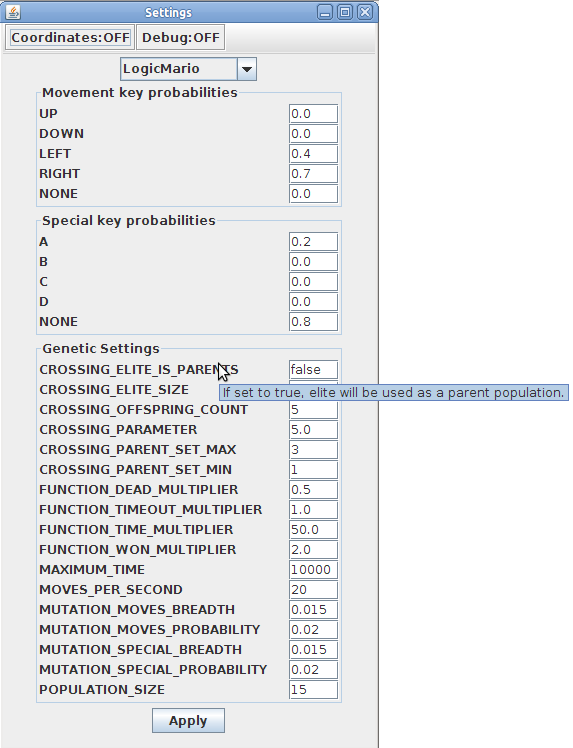
\includegraphics[width=4in]{obrazki/config1.png}
		\caption{Panel Konfiguracyjny.}
		\label{fig:config1}
	\end{figure}
	Trzecia grupa parametr�w s� to parametry algorytmu genetycznego (grupa \textit{Genetic Settings}). Po umieszczeniu kursora myszy nad nazw� parametru wy�wietlany jest jego opis s�owny. Uzytkownik mo�e zmieni� poszczeg�lne parametry. W wypadku zmiany parametr�w wymagaj�cych ponownego uruchomienia aplikacji, wy�wietlone zostaje okno pytaj�ce o potwierdzenie operacji.
	\newline
	Poniewa� algorytm genetyczny jest niezale�ny od stosowanej logiki gry, mo�liwe jest rozbudowywanie aplikacji o dodawanie w�asnych klas dziedzicz�cych po klasie Logic. U�ytkownik ma mo�liwo�� zmiany logiki w panelu ustawie�, za pomoc� listy na g�rze okna ustawie�.
	Dwa dodatkowe przyciski w panelu konfiguracyjnym (``Coordinates'' oraz ``Debug'') s�u�� do w��czenia wy�wietlania informacji o obiektach takich jak ich po�o�enie w przestrzeni, lub informacji o stanie gry. Mog� one okaza� si� przydatne przy tworzeniu w�asnych map, b�d� pisaniu w�asnej logiki gry.
\end{par}
\subsection{Widok Populacji i Chromosomu}
\begin{par}
	Podczas dzia�ania algorytmu genetycznego nawet w trybie przyspieszonym, u�ytkownik mo�e �ledzi� post�py w oknie ``Population'' dost�pnym z menu (Rys. \ref{fig:populacja}).
	Zawiera ono list� aktualnie dost�pnych osobnik�w w populacji i wy�wietla kr�tkie podsumowanie dotycz�ce przebiegu danego osobnika w symulacji gry. Kolejno \textit{Result} oznacza wynik ko�cowy po zako�czeniu przebiegu, \textit{Score} dotyczy sumy wszystkich zebranych punkt�w na mapie. Warto�� \textit{Time} oznacza czas przebiegu danego chromosomu w milisekundach.
	Ostatecznie \textit{Final Score} jest warto�ci� funkcji przystosowania przeliczon� przez algorytm. Je�li dany osobnik jeszcze nie wzi�� udzia�u w przebiegu gry, wy�wietlany jest komunikat ``State not Set''. Po zaznaczeniu dowolnego osobnika u�ytkownik ma mo�liwo�� tymczasowego uruchomienia przej�cia za pomoc� przycisku ``Run selected gene''. Po zaznaczeniu osobnika i wci�ni�ciu przycisku ``Show details'' wy�wietlane zostaje okno podgl�du chromosomu - Rys. \ref{fig:chromosom}.

	\begin{figure}[!h]
		\centering
		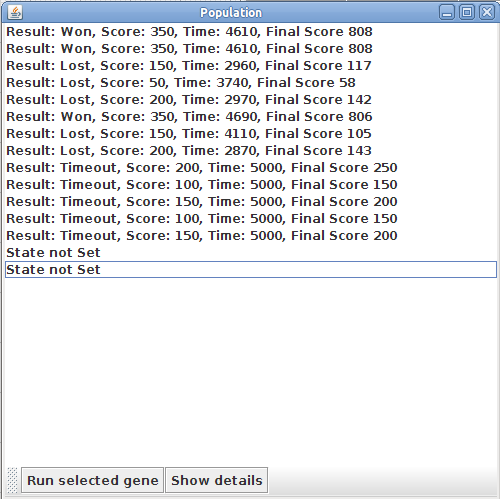
\includegraphics[width=4in]{obrazki/populacja.png}
		\caption{Okno populacji.}
		\label{fig:populacja}
	\end{figure}


	\begin{figure}[!h]
		\centering
		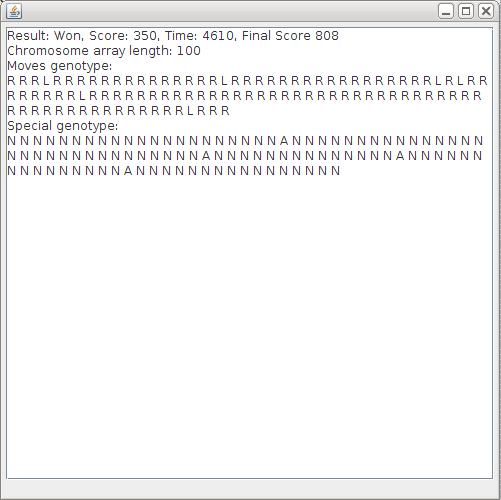
\includegraphics[width=4in]{obrazki/chromosom.png}
		\caption{Okno szczeg��w chromosomu.}
		\label{fig:chromosom}
	\end{figure}
	\FloatBarrier
\end{par}


\subsection{Edytor Map}
\begin{par}
	Przy testowaniu r�nych ustawie� algorytmu genetycznego przydatnym narz�dziem mo�e okaza� si� edytor map. 
	Ustawienia algorytmu, szczeg�lnie dotycz�ce prawdopodobie�stwa wylosowania akcji w du�ej mierze zale�� od typu mapy. 
	U�ytkownik mo�e otworzy� okno edytora map wybieraj� opcj� ``Map Editor'' z menu g��wnego okna aplikacji.
	Po otworzeniu edytora map domy�lnie wczytywana jest bie��ca mapa z symulatora gry, dzi�ki czemu mo�na dokona� szybkich edycji je�li koniecznie jest sprawdzenie dzia�ania algorytmu z pewnym wariantem, lub dodatkowym obiektem na mapie.
	Opr�cz tego wszystkie mapy zapisywane s� w prostym formacie tekstowym, dzi�ki czemu mo�liwe jest generowanie map przy pomocy program�w trzecich, lub skrypt�w - zostawia to furtk� dla bardziej zaawansowanych u�ytkownik�w na generowanie du�ych poziom�w, lub wykorzystanie algorytm�w tworz�cych losowe tereny.
	Przyk�adowy plik z map� mo�e wygl�da� nast�puj�co:
	\begin{lstlisting}
		Terrain 122 361 239 27
		Terrain 110 211 25 151
		Terrain 355 201 28 165
		Actor 140 295 20 32
		BonusCoin 202 328 18 30 25
		BonusCoin 248 330 16 27 25
		BonusWin 327 236 18 36 25
		BonusLose 313 311 33 40 0
	\end{lstlisting}

	Pierwszym elementem ka�dego wiersza jest nazwa klasy.
	Kolejne warto�ci to punkt oznaczaj�cy po�o�enie lewego g�rnego rogu obiektu, oraz jego szeroko�� i wysoko��.
	W wypadku obiekt�w klasy \textit{Bonus} ostatnia liczba oznacza warto�� punktow�. 
	Poniewa� nie by�o powodu aby przechowywa� mapy jako dane binarne - samo wczytywanie mapy nie spowalnia aplikacji oraz nie jest wykonywane cz�sto - otwarty format pozosta� jako obowi�zuj�cy w systemie.
\end{par}
\begin{par}
	\begin{figure}[!h]
	\centering
	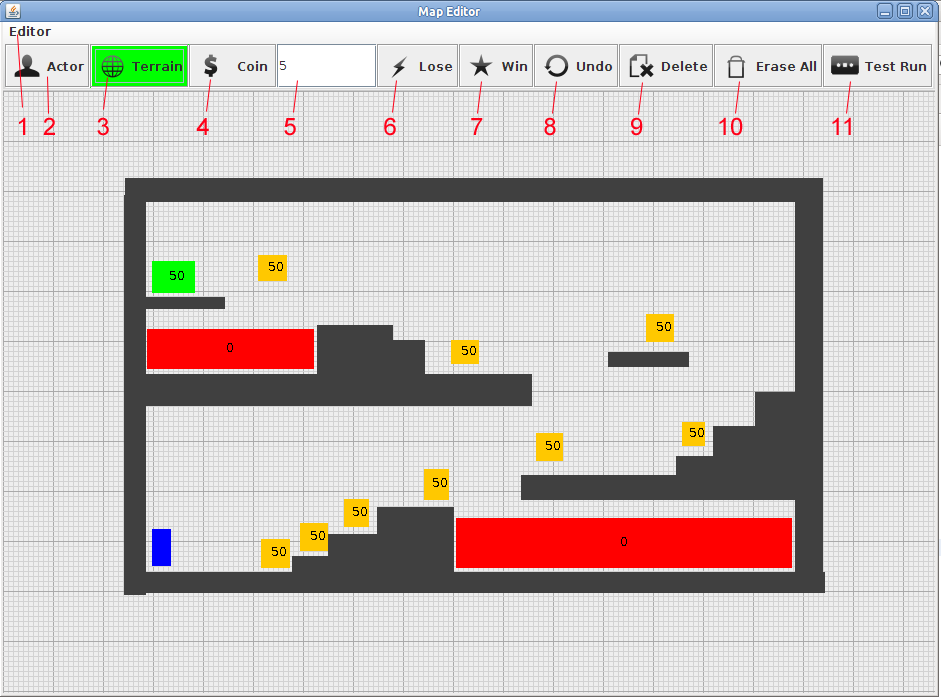
\includegraphics[width=5.5in]{obrazki/map_editor.png}
	\caption{Okno edytora map.}
	\label{fig:map_editor}
	\end{figure}
	Samo okno edytora map sk�ada si� z menu oraz paska narz�dzi. Pos�ugiwanie si� wi�kszo�ci� narz�dzi jest podobne:
	\begin{itemize}
	\item U�ytkownik aby narysowa� obszar wybiera odpowiedni typ obiektu z paska narz�dzi, a nast�pnie trzymaj�c lewy przycisk myszy, wyznacza prostok�tny obszar.
	\item Po klikni�ciu na dowolny obiekt lewym przyciskiem myszy, zostaje on zaznaczony, dzi�ki czemu u�ytkownik mo�e �atwo usuwa� z mapy niepotrzebne obiekty.
	\item Prawy przycisk myszy s�u�y do przesuwania mapy - analogicznie do trybu ``MouseCam'' w module symulacyjnym.
	\end{itemize}
	Poni�ej zostan� opisane poszczeg�lne elementy edytora.
	\begin{enumerate}
		\item Menu edytora pozwalaj�ce u�ytkownikowi na wczytanie mapy z pliku, b�d� zapis bie��cej mapy do pliku na dysku. W obu przypadkach wy�wietlane jest okno dialogowe potwierdzaj�ce operacj�.
		\item Przycisk uaktywniaj�cy obiekt aktora. Po wybraniu przycisku obiekty tworzone przez u�ytkownika b�d� obiektami aktora. Na mapie jednocze�nie mo�e by� utworzonych wiele obiekt�w aktora. Poniewa� w za�o�eniach nie jest powiedziane i� gra mo�e zawiera� tylko jeden obiekt sterowany przez u�ytkownika istnieje mo�liwo�� dodania na mapie wielu aktor�w - mo�liwe jest napisanie logiki wykorzystuj�cej wi�cej ni� jeden obiekt aktora.
		\item Obiekt Terrain odpowiada za statyczny teren gry. O ile interpretacja kolizji aktora z obiektem tego typu jest pozostawiona do interpretacji dla tw�rcy logiki, to g��wnym za�o�eniem obiektu Terrain mia�o by� ograniczanie ruchu postaci po mapie.
		\item Przycisk Coin odpowiada za umieszczanie obiekty BonusCoin daj�cych punkty.
		\item Warto�� w polu tekstowym pozwala na ustalenie warto�ci jak� ma mie� nast�pny stworzony przez u�ytkownika obiekt BonusCoin.
		\item Przycisk Lose odpowiada za umieszczanie na mapie obiekt�w typu BonusLose.
		\item Przycisk Win odpowiada za umieszczanie na mapie obiekt�w typu BonusWin.
		\item Przycisk Undo usuwa ostatnio stworzony obiekt z mapy.
		\item Przycisk Delete usuwa aktualnie zaznaczony na mapie obiekt.
		\item Je�li u�ytkownik chce usun�� wszystkie elementy z mapy i rozpocz�� tworzenie mapy od pocz�tku, mo�e u�y� do tego przycisku Erase All kt�ry usuwa wszystkie obiekty z edytora map. Przed wykonaniem akcji u�ytkownik zatwierdza akcj� w oknie dialogowym.
		\item Przycisk Test Run s�u�y do za�adowania bie��cej mapy z edytora do �rodowiska gry. Je�li aktualnie system pracuje w trybie treningu populacji, konieczne jest rozpocz�cie algorytmu od pocz�tku. Mapa zostaje zapisana na dysk jako plik tymczasowy. Przed wykonaniem akcji u�ytkownik zatwierdza akcj� w oknie dialogowym.
		
	\end{enumerate}
	
\end{par}


\chapter{Podsumowanie}
\begin{par}
	Podczas implementacji systemu wynik�y problemy dotycz�ce wielow�tkowo�ci w j�zyku java, a dok�adnie wsp�dzielenie zasob�w przez w�tek gry, oraz w�tek zwi�zany z wy�wietlaniem interfejsu u�ytkownika. Podczas pracy nad systemem du�ym problemem by�o cz�ste pojawianie si� wyj�tku ``ConcurrentModificationException'' dotycz�cego jednoczej modyfikacji listy element�w gry przez dwa w�tki. Domy�lnym rozwi�zaniem jest umieszczenie modyfikacji listy w bloku synchronized{ }, co zmniejszy�o cz�stotliwo�� wyst�powania wyj�tku, jednak dopiero zastosowanie zmiennej typu mutex rozwi�za�o ca�kowicie problem. Przypuszcza si� i� mo�e by� to pewna w�a�ciwo�� biblioteki Swing kt�ra w po��czeniu z pewnymi b��dami projektowymi po stronie implementacji system, sprawia�a problem.
\end{par}
\begin{par}
	Przy uruchamianiu aplikacji na wolniejszych komputerach mo�na by�o zauwa�y� pewien spadek p�ynno�ci gry. Problem ten mo�na by�oby rozwi�za� korzystaj�c z gotowych bibliotek graficznych (np. OpenGL), kt�re dzia�aj� szybciej ni� w�asna implementacja warstwy graficznej. Innym usprawnieniem mog�oby by� u�ycie biblioteki SWT zamiast biblioteki Swing, dzi�ki czemu wygl�d aplikacji lepiej pasowa�by do danego systemu operacyjnego - aplikacje okienkowe napisane w bibliotece SWT przypominaj� wygl�dem standardowe aplikacje systemu. Je�li chodzi o sam j�zyk programowania to Java w zupe�no�ci spe�nia wymagania systemu.
\end{par}
\begin{par}
	Sam system genetyczny daje do�� dobre wyniki na prostych mapach (np. ukierunkowanych). Du�o gorzej radzi sobie z logik� wymagaj�c� poruszania si� w 4 kierunkach (np. LogicLabirynth). Usprawnieniem systemu mog�oby by� wykorzystanie algorytm�w przeszukuj�cych przestrze� rozwi�za� (np. algorytm przeszukuj�cy A*) wraz z algorytmem genetycznym. Sam algorytm genetyczny znajduje rozwi�zanie za pomoc� standardowego podej�cia, jednak je�li celem systemu by�oby najszybsze rozwi�zanie danej gry, algorytm przeszukuj�cy z pewn� heurystyk� mo�e okaza� si� lepszym podej�ciem. Du�� zalet� systemu jest jego elastyczno�� - mo�liwo�� dodawania w�asnych map oraz logik do systemu. Z perspektywy czasu autor systemu jest zadowolony z otrzymanych rezultat�w, jednak przy ponownej pr�bie implementacji skorzysta�by z innych narz�dzi i bibliotek, szczeg�lnie je�li chodzi o warstw� wizualizacyjn�.
\end{par}

\nocite{*} %wszystkie wpisy w bibliografi
\bibliographystyle{unsrt} %{latex8} posortowane wzgledem wystepowania
\bibliography{bibliografia}%

\addtocontents{toc}{\contentsline {chapter}{Bibliografia}{\thepage}{}}
\listoftables
\addtocontents{toc}{\contentsline {chapter}{Spis tabel}{\thepage}{}}
\listoffigures
\addtocontents{toc}{\contentsline {chapter}{Spis rysunków}{\thepage}{}}
\lstlistoflistings
\addtocontents{toc}{\contentsline {chapter}{Spis listingów}{\thepage}{}}
\listofalgorithms % w zaleznosci od kompilatora i wersji klasy moga wystapic bledy przy kompilacji
\addtocontents{toc}{\contentsline {chapter}{Spis algorytmów}{\thepage}{}}

%\biblioteka{tak} % tak/nie
\end{document}
